\chapter{Implementacija i korisničko sučelje}
		
		
		\section{Korištene tehnologije i alati}
		
			 Za međusobnu komunikaciju tijekom izrade naše KuhajIT aplikacije korištene su dvije aplikacije: \textcolor{blue}{\underline{\href{https://discord.com/download}{\textcolor{blue}{Discord}}}}\footnote{\url{https://discord.com/download}} i \textcolor{blue}{\underline{\href{https://www.whatsapp.com/download/}{\textcolor{blue}{WhatsApp}}}}\footnote{\url{https://www.whatsapp.com/download/}}.
			 		 
WhatsApp je aplikacija za razmjenu poruka koja omogućava korisnicima slanje tekstualnih poruka, medijskih datoteka (poput slika, videa i audio zapisa), te poziva i video poziva putem internetskog povezivanja. Mi smo ju koristili za interno dogovaranje o onome što je iduće potrebno obaviti te o terminima sastanaka uživo.

Discord je platforma za komunikaciju putem interneta koja je prvobitno dizajnirana za zajednice igrača, ali se brzo proširila na različite druge vrste korisnika. Omogućava korisnicima stvaranje privatnih ili javnih "servera" (prostorija) gdje se mogu razgovarati putem teksta, glasa ili videa. Mi smo ju koristili za hitne sastanke u slučaju da je netko od članova pri izradi naišao na problem bilo kakve vrste i trebala mu je asistencija drugog člana tima.

Upravljanje izvornim kodom ostvareno je sustavom \textcolor{blue}{\underline{\href{https://git-scm.com/downloads}{\textcolor{blue}{Git}}}}\footnote{\url{https://git-scm.com/downloads}}, a udaljeni repozitorij
čitavog projekta dostupan nam je bio na web platformi \textcolor{blue}{\underline{\href{https://github.com/}{\textcolor{blue}{GitHub}}}}\footnote{\url{https://github.com/}}.

			Git je sustav za upravljanje verzijama koji se široko koristi u razvoju softvera. Omogućava programerima i timovima praćenje promjena u izvornom kodu tijekom vremena, praćenje različitih verzija projekta te suradnju među programerima, te smo ga mi na taj način koristili.
			
			GitHub je web platforma za upravljanje verzijama i suradnju na razvoju softvera. Osnovna funkcionalnost GitHub-a leži u Git-u, koji omogućuje razvojnom timu praćenje promjena u izvornom kodu tijekom vremena. 
			Za izradu svih UML dijagrama korišten je alat \textcolor{blue}{\underline{\href{https://astah.net/downloads/}{\textcolor{blue}{Astah UML}}}}\footnote{\url{https://astah.net/downloads/}}.
			
Astah UML je vrsta alata koji pomaže programerima, analitičarima sustava i drugima da vizualiziraju, modeliraju i dokumentiraju arhitekturu softvera. Podržava različite vrste dijagrama, od kojih smo mi koristili dijagrame razreda, stanja, aktivnosti, komponenti, dijagrame obrazaca uporabe te sekvencijske dijagrame.

Odabrana razvojna okruženja pri izradi naše aplikacije bila su \textcolor{blue}{\underline{\href{https://code.visualstudio.com/Download}{\textcolor{blue}{Visual Studio Code}}}}\footnote{\url{https://code.visualstudio.com/Download}} za frontend i \textcolor{blue}{\underline{\href{https://www.eclipse.org/downloads/}{\textcolor{blue}{Eclipse}}}}\footnote{\url{https://www.eclipse.org/downloads/}} za backend.


Visual Studio Code je razvojno okruženje za pisanje koda razvijen od strane Microsofta. Odlikuje ga bogata podrška za web tehnologije, kao što su HTML, CSS, JavaScript, Typescript itd.

Eclipse je razvojno okruženje koje podržava brojne programske jezike, a neki od njih su: Java, C++, PHP, Python, Ruby...

Kako je već prije navedeno, za razvoj frontenda naše aplikacije koristili smo \textcolor{blue}{\underline{\href{https://www.javascript.com/}{\textcolor{blue}{JavaScript}}}}\footnote{\url{https://www.javascript.com/}} i \textcolor{blue}{\underline{\href{https://react.dev/}{\textcolor{blue}{React}}}}\footnote{\url{https://react.dev/}}.

JavaScript je visokoprogamski jezik koji se često koristi za izgradnju dinamičkih web stranica i web aplikacija, razvijen u Netscape Communications Corporation-u. Najčešće se koristi za programiranje na strani klijenta.

React je JavaScript biblioteka za izgradnju korisničkih sučelja, koju karakterizira komponentna arhitektura koja olakšava organizaciju koda i upravljanje stanjem aplikacije.

Za razvoj backenda naše aplikacije korišten je \textcolor{blue}{\underline{\href{https://spring.io/projects/spring-boot/}{\textcolor{blue}{Spring Boot}}}}\footnote{\url{https://spring.io/projects/spring-boot/}}.

Spring Boot je open-source okvir za izgradnju Java web aplikacija i mikroservisa, dio šireg Spring ekosustava. Posebno je fokusiran na pojednostavljenje konfiguracije, ubrzanje razvoja i olakšavanje izgradnje samostalnih aplikacija.


Baza podataka razvijena je pomoću sustava za upravljanje bazom podataka \textcolor{blue}{\underline{\href{https://www.postgresql.org/download/}{\textcolor{blue}{PostgreSQL}}}}\footnote{\url{https://www.postgresql.org/download/}}.
			\eject 
			
		\section{Ispitivanje programskog rješenja}
			
			\subsection{Ispitivanje komponenti}
\textbf{Test 1: Uspješna registracija} \\
Provedeno je testiranje uspješne registracije novog, dotad neregistriranog korinsika u sustav. Registracija je uspješna ako ne baca iznimku i ako metoda "registerUser" klase UserService vraća istinitu vrijednost. Na slikama ispod prikazani su test uspješne registracije i metoda "registerUser" klase UserService, kao i potvrda uspješne provedbe testa.

		\begin{figure}[H]
			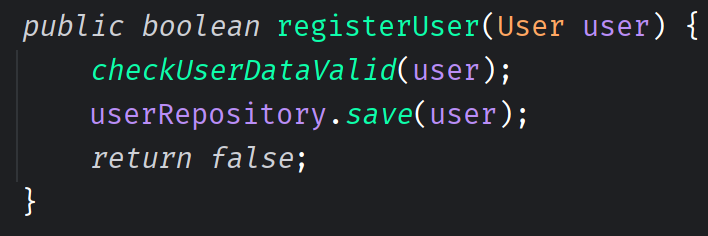
\includegraphics[scale=0.4]{slike/registerUser.PNG} %veličina slike u odnosu na originalnu datoteku i pozicija slike
			\centering
			\caption{Metoda "registerUser" klase UserService}
			\label{Metoda "registerUser" klase UserService}
		\end{figure}
		
				\begin{figure}[H]
			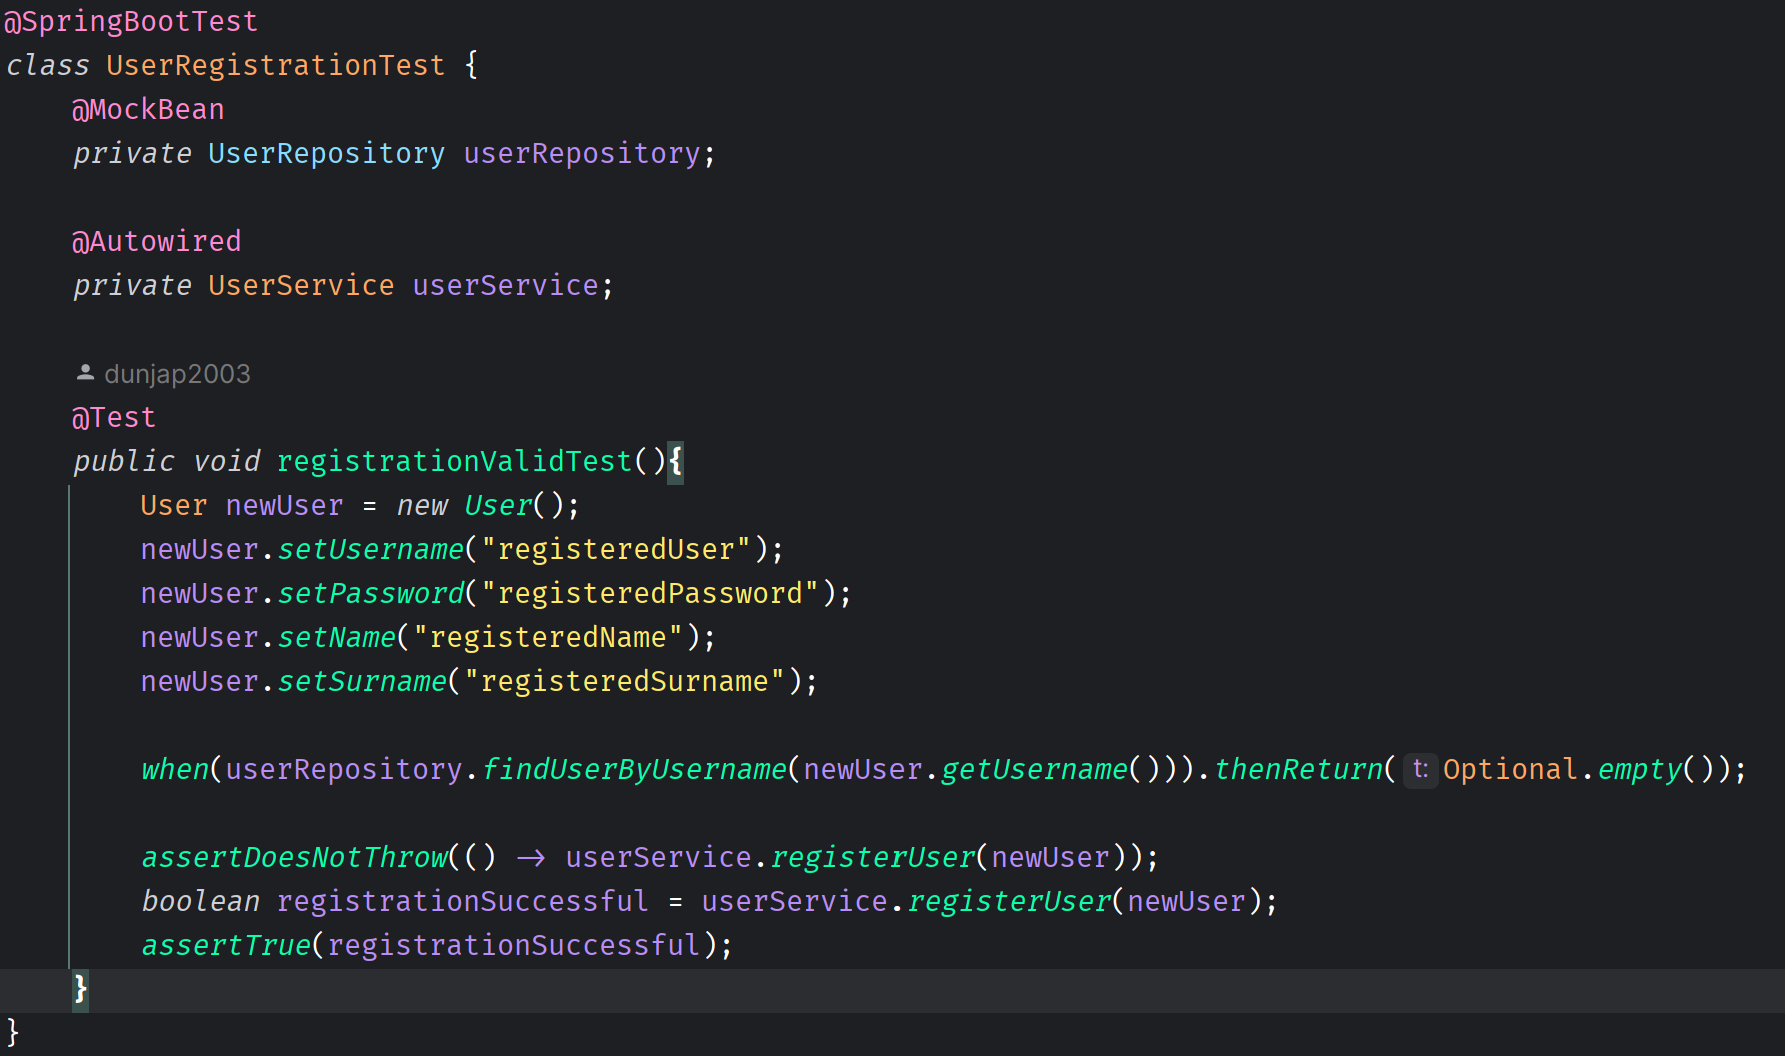
\includegraphics[scale=0.4]{slike/userRegistrationTest.PNG} %veličina slike u odnosu na originalnu datoteku i pozicija slike
			\centering
			\caption{Test uspješne registracije korisnika}
			\label{Test uspješne registracije korisnika}
		\end{figure}
		
					\begin{figure}[H]
			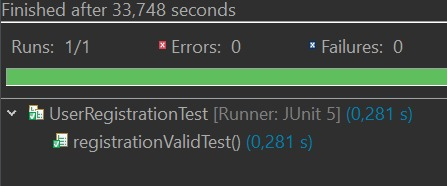
\includegraphics[scale=0.4]{slike/JUnit_register.JPG} %veličina slike u odnosu na originalnu datoteku i pozicija slike
			\centering
			\caption{Potvrda uspješnog izvođenja testa registracije}
			\label{Potvrda uspješnog izvođenja testa registracije}
		\end{figure}
		
		
\textbf{Test 2: Uspješna prijava korisnika} \\
Provedeno je testiranje ispravne prijave korisnika koji je registriran i prisutan u bazi. Prijava je uspješna ako metoda "loginUser" klase UserService ne vraća null vrijednost i ako su svi atributi prethodno stvorenog objekta korisnika i atributi korisnika koji je spremljen u oponašan repozitorij korisnika jednaki. Na slikama ispod prikazani su test uspješne prijave korisnika i metoda "loginUser" klase UserService.

				\begin{figure}[H]
			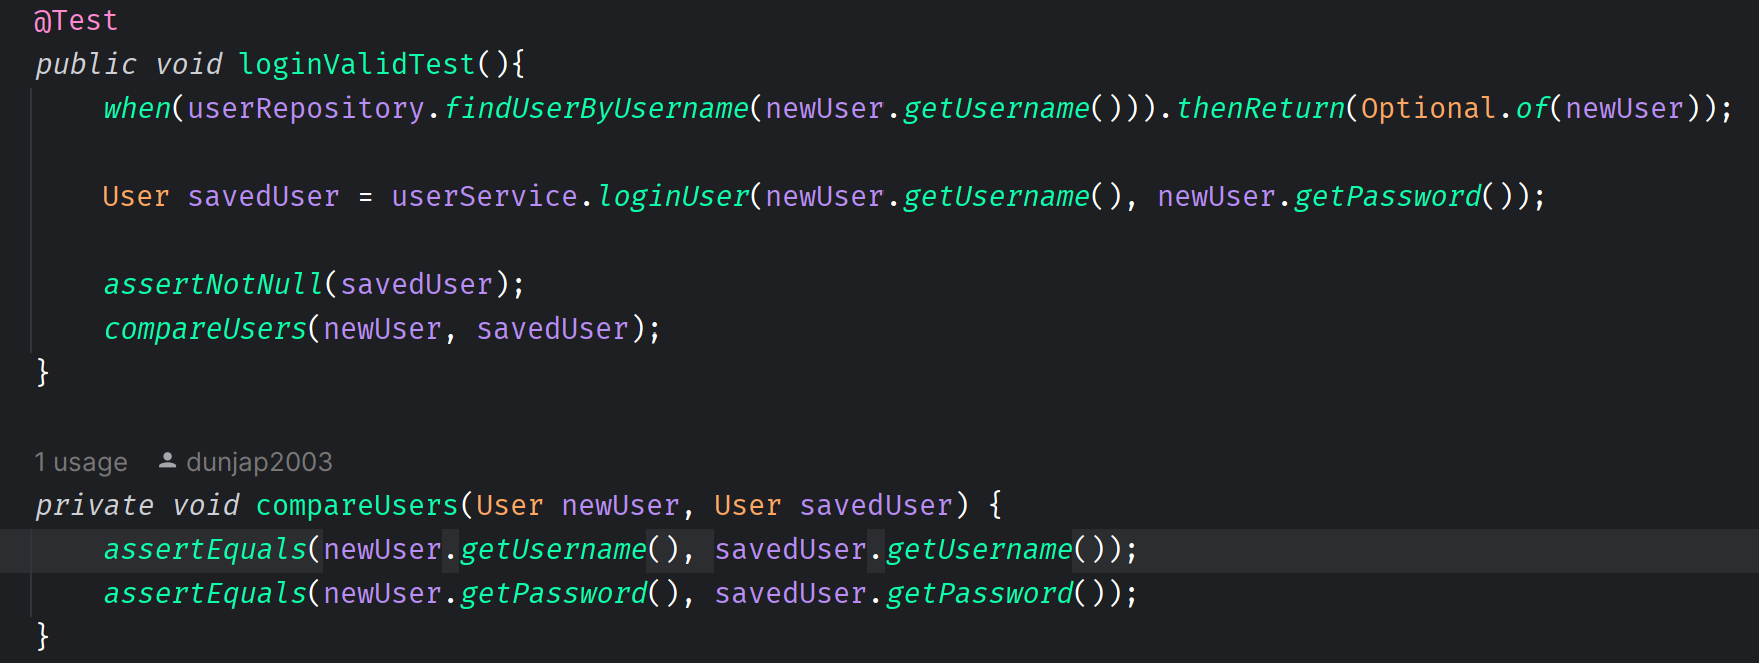
\includegraphics[scale=0.4]{slike/loginValidTest.PNG} %veličina slike u odnosu na originalnu datoteku i pozicija slike
			\centering
			\caption{Test uspješne prijave korisnika}
			\label{Test uspješne prijave korisnika}
		\end{figure}
		
						\begin{figure}[H]
			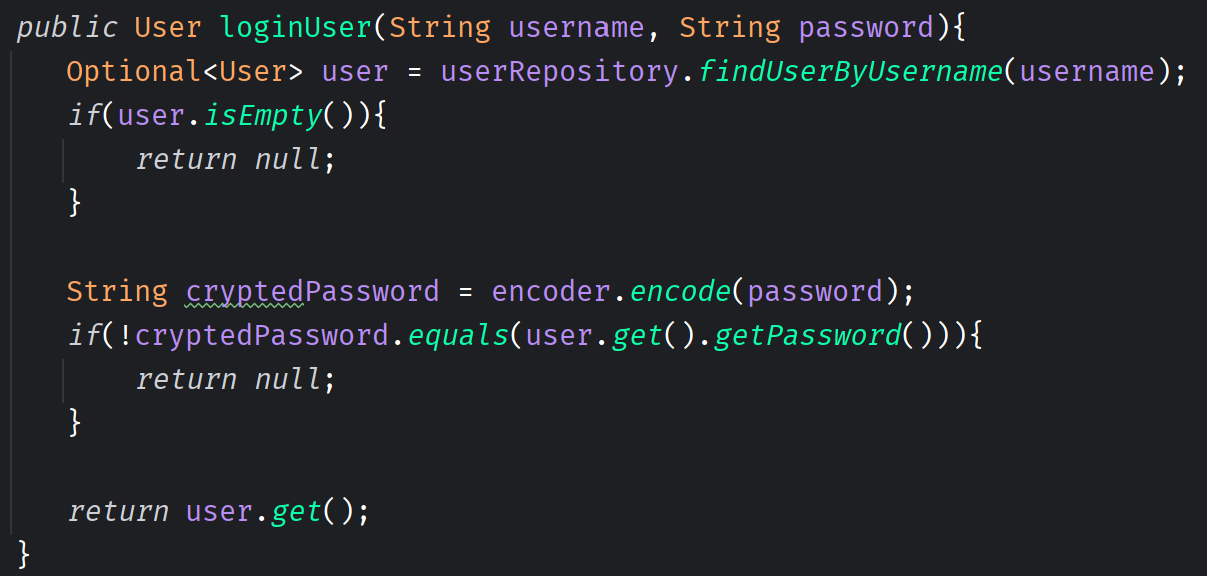
\includegraphics[scale=0.4]{slike/loginUser.PNG} %veličina slike u odnosu na originalnu datoteku i pozicija slike
			\centering
			\caption{Metoda "loginUser" klase UserService}
			\label{Metoda "loginUser" klase UserService}
		\end{figure}
		
\textbf{Test 3: Neuspješna prijava korisnika (nepostojeće korisničko ime)} \\
Provedeno je testiranje neuspješne prijave korisnika zbog unosa neispravnog korisničkog imena, tj. korisničkog imena koje se ne nalazi u oponašanom repozitoriju korisnika koji je simuliran u sklopu testiranja. Neuspješna prijava korisnika manifestira se kroz dohvaćenu null vrijednost prilikom dohvaćanja traženog korisnika iz oponašanog repozitorija korisnika. Na slici ispod prikazan je test neuspješne prijave korisnika zbog nepostojećeg korisničkog imena. Metoda "loginUser" klase UserService prikazana je u slici iznad.

				\begin{figure}[H]
			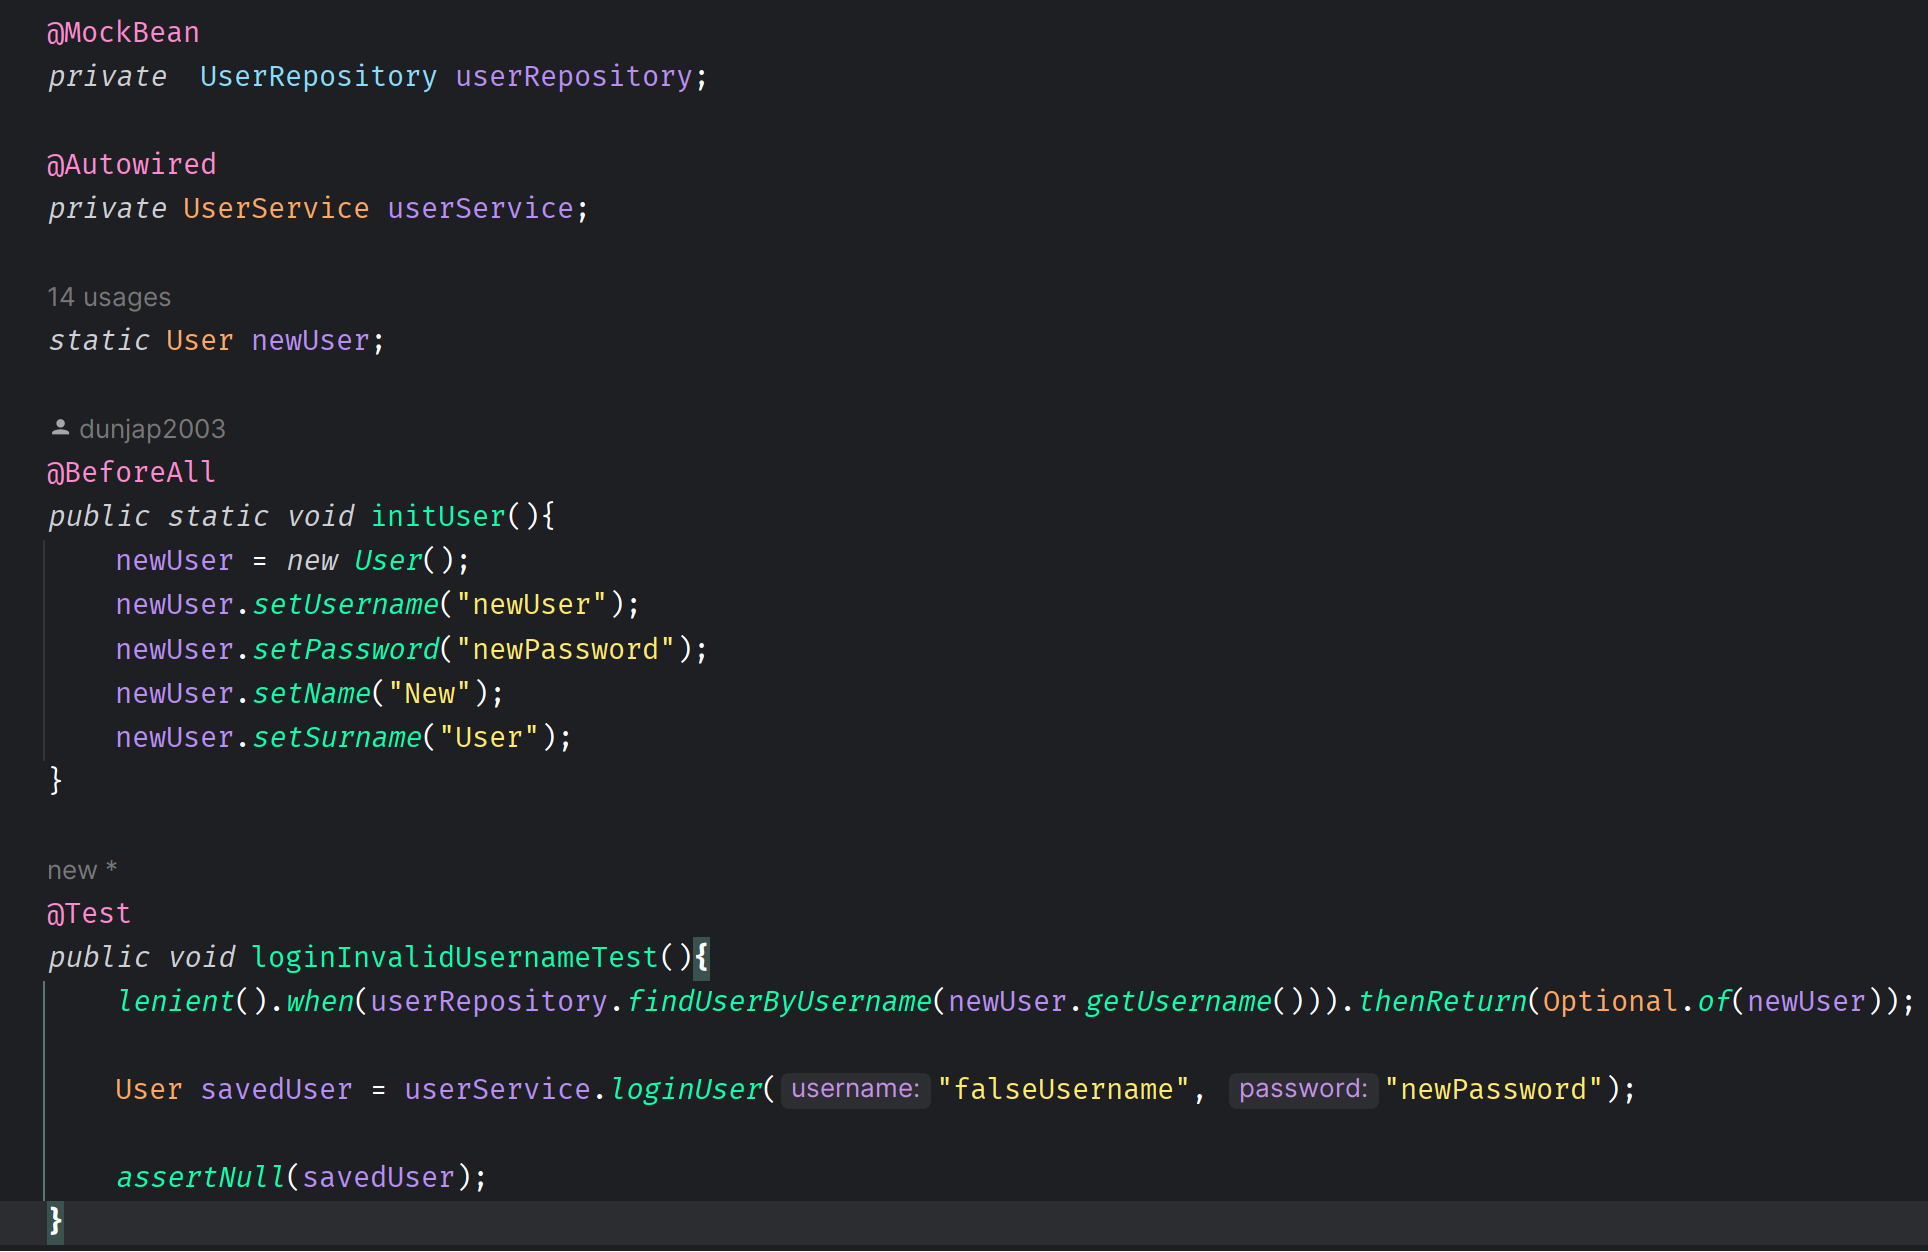
\includegraphics[scale=0.4]{slike/loginInvalidUsernameTest.PNG} %veličina slike u odnosu na originalnu datoteku i pozicija slike
			\centering
			\caption{Test neuspješne prijave korisnika zbog nepostojećeg korisničkog imena}
			\label{Test neuspješne prijave korisnika zbog nepostojećeg korisničkog imena}
		\end{figure}
		
\textbf{Test 4: Neuspješna prijava korisnika (pogrešna lozinka)} \\
Provedeno je testiranje neuspješne prijave korisnika zbog unosa ispravnog korisničkog imena, ali neispravne lozinke koja bi omogućila pristup profilu s tim korisničkim imenom. Neuspješna prijava korisnika zbog neispravne lozinke manifestira se kroz dohvaćenu null vrijednost prilikom usporedbi lozinki spremljenog korisnika s tim korisničkim imenom i upisane lozinke za to korisničko ime. Na slici ispod prikazan je test neuspješne prijave korisnika zbog upisane neispravne lozinke. Metoda "loginUser" klase UserService prikazana je u slici iznad.

				\begin{figure}[H]
			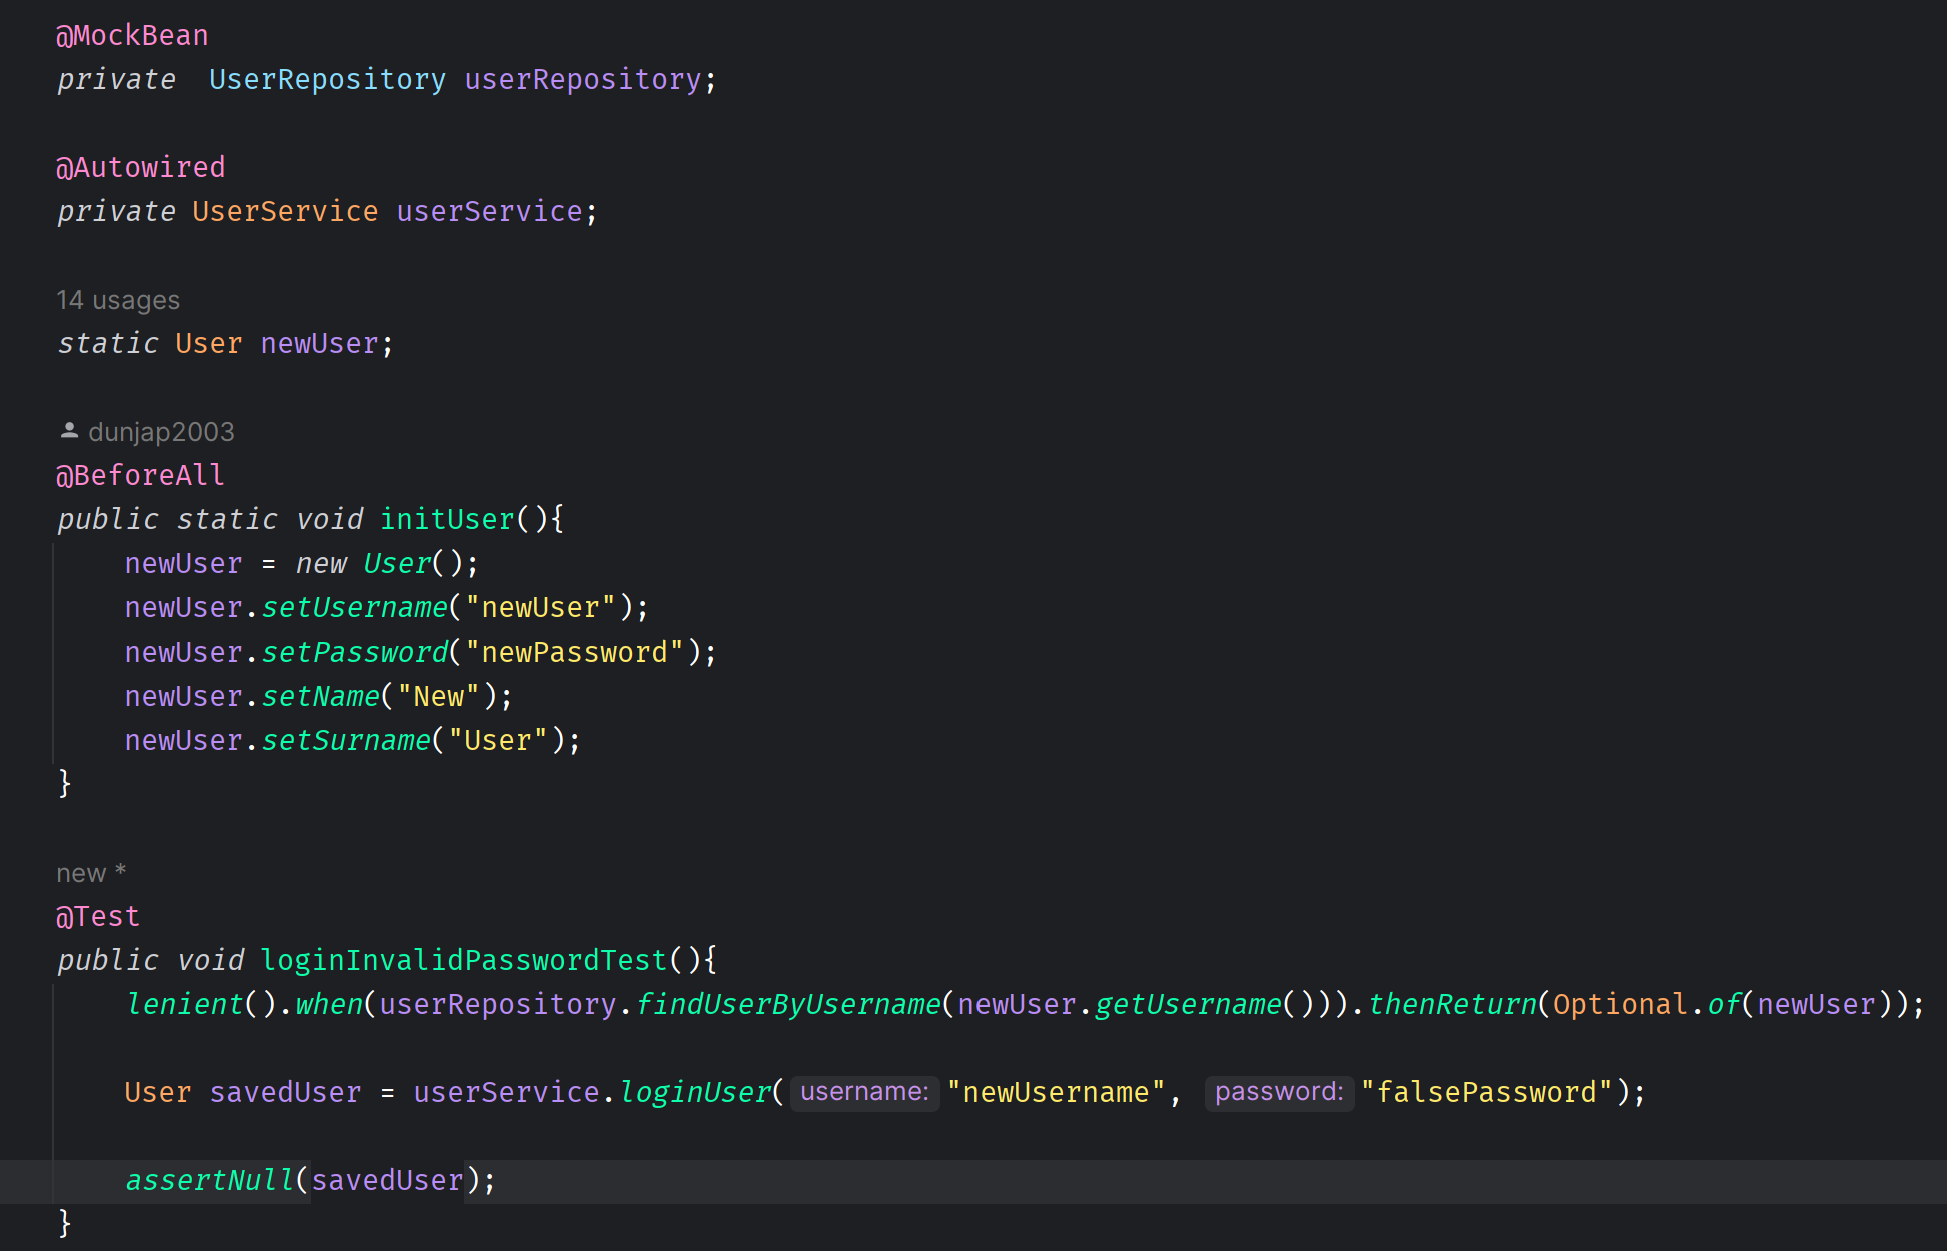
\includegraphics[scale=0.4]{slike/loginInvalidPasswordTest.PNG} %veličina slike u odnosu na originalnu datoteku i pozicija slike
			\centering
			\caption{Test neuspješne prijave korisnika zbog unosa neispravne lozinke}
			\label{Test neuspješne prijave korisnika zbog unosa neispravne lozinke}
		\end{figure}
		
		Na slici ispod prikazane su potvrde uspješnog izvođenja testova vezanih uz login.
		
			\begin{figure}[H]
			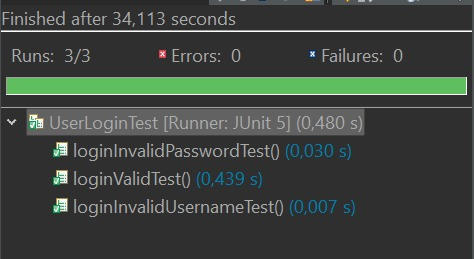
\includegraphics[scale=0.4]{slike/JUnit_login.JPG} %veličina slike u odnosu na originalnu datoteku i pozicija slike
			\centering
			\caption{Potvrda uspješnog izvođenja testova vezanih uz login}
			\label{Potvrda uspješnog izvođenja testova vezanih uz login}
		\end{figure}
			
\textbf{Test 5: Uspješno dohvaćanje podataka o korisniku iz baze podataka} \\

Provedeno je testiranje uspješnog dohvaćanja podataka o korisniku iz baze podataka. Dohvaćanje podataka o korisniku iz baze podataka je uspješno ako metoda "loadUserByUsername" klase UserService vrati objekt korisnika koji je pronađen putem korisničkog imena i ako su atributi korisnika dohvaćenog iz oponašanog repozitorija korisnika i atributi onog korisnika koji je inicijalno spremljen u oponašani repozitorij jednaki. Na slikama ispod prikazani su test uspješnog dohvaćanja podataka o korisniku iz baze podataka te metoda "loadUserByUsername" klase UserService, kao i potvrda uspješno izvedenog testa o dohvaćanju podataka o korisniku iz baze podataka.

				\begin{figure}[H]
			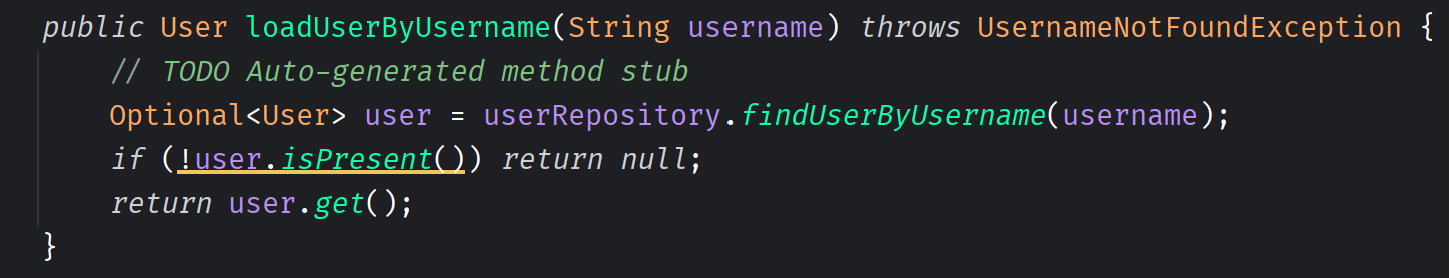
\includegraphics[scale=0.4]{slike/loadUserByUsername.PNG} %veličina slike u odnosu na originalnu datoteku i pozicija slike
			\centering
			\caption{Metoda "loadUserByUsername" klase UserService}
			\label{Metoda "loadUserByUsername" klase UserService}
		\end{figure}
		
						\begin{figure}[H]
			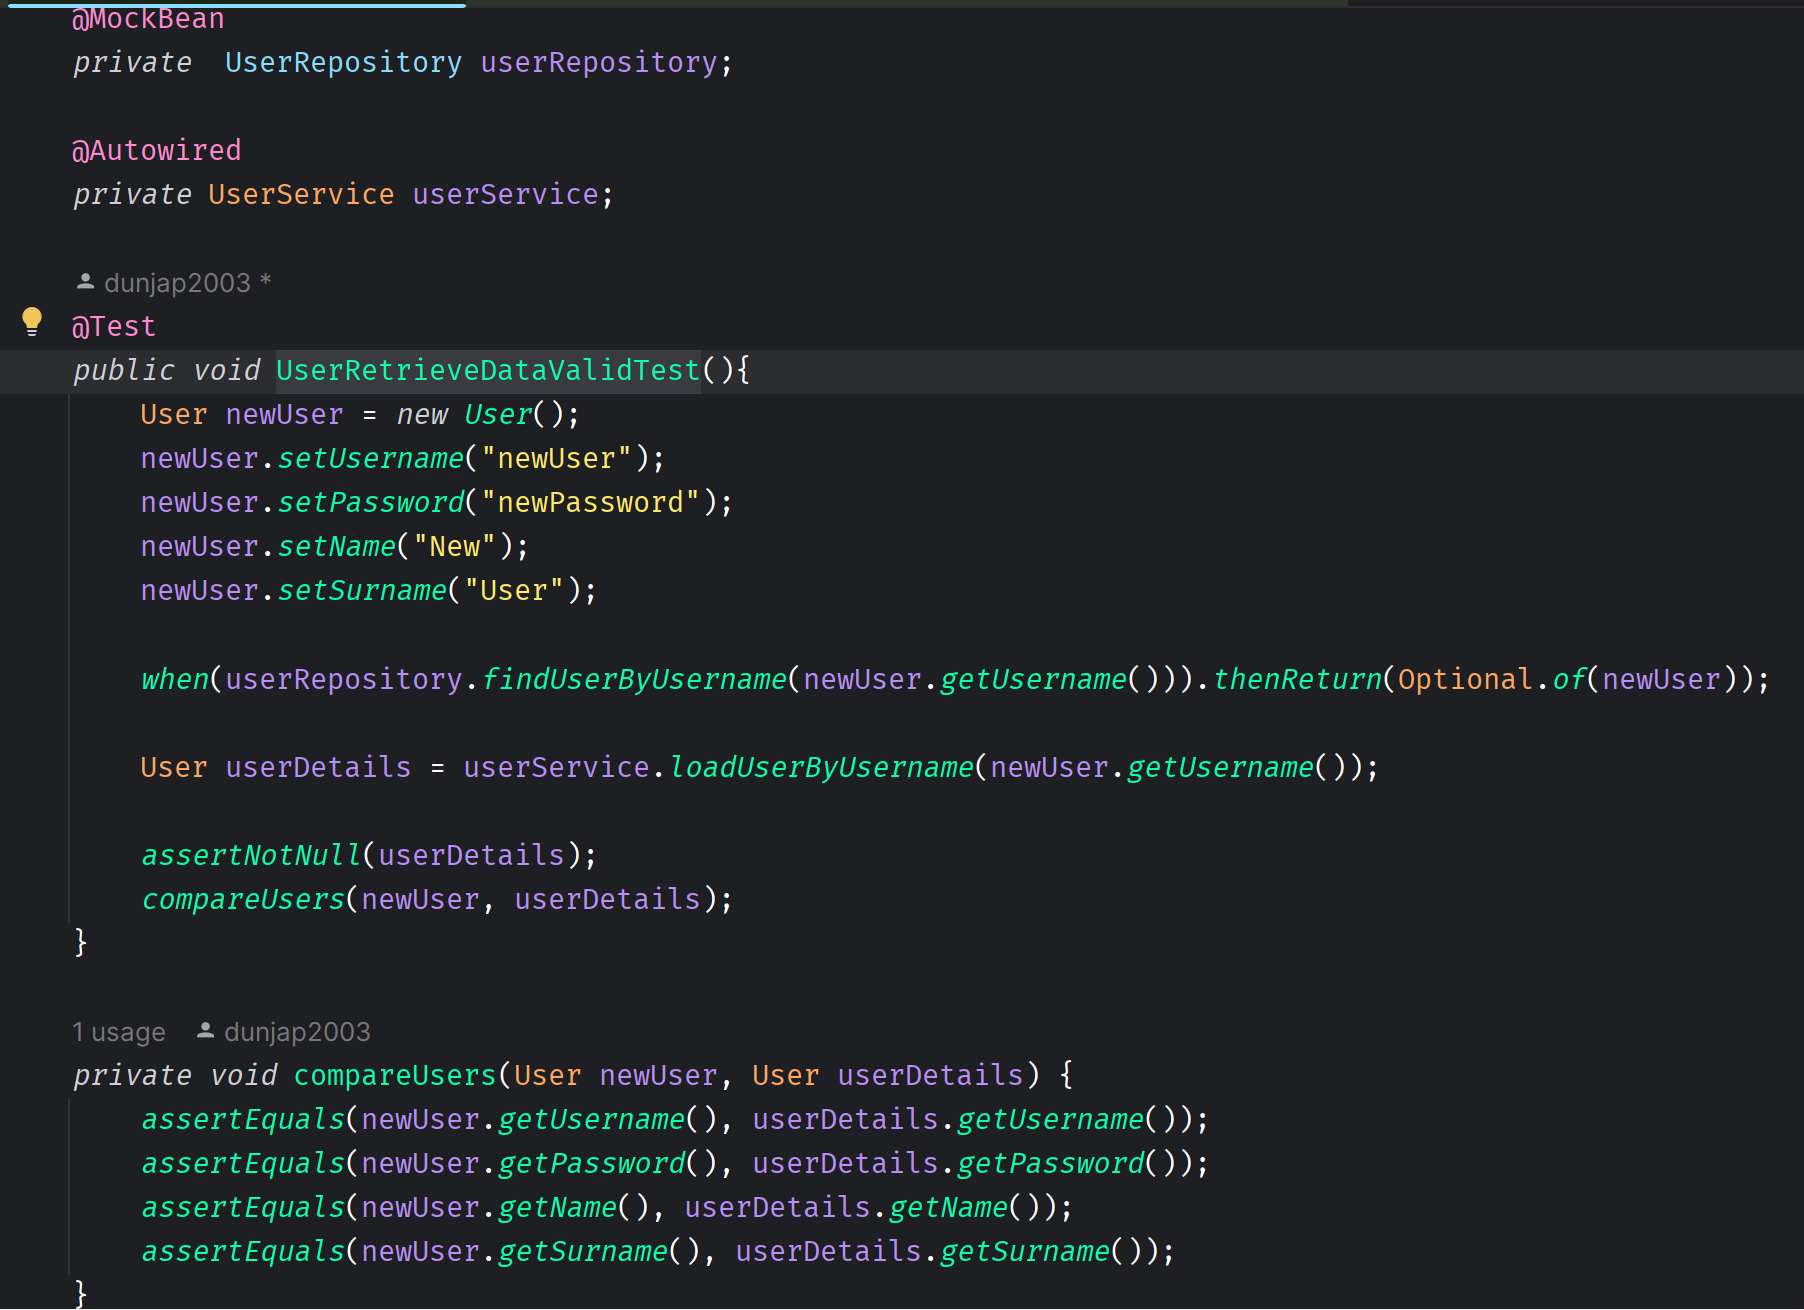
\includegraphics[scale=0.4]{slike/userRetrieveDataValidTest.PNG} %veličina slike u odnosu na originalnu datoteku i pozicija slike
			\centering
			\caption{Test uspješnog dohvaćanja podataka o korisniku na temelju korisničkog imena iz baze podataka}
			\label{Test uspješnog dohvaćanja podataka o korisniku na temelju korisničkog imena iz baze podataka}
		\end{figure}
		
			\begin{figure}[H]
			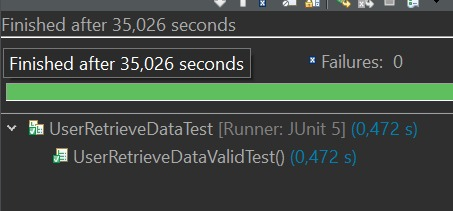
\includegraphics[scale=0.4]{slike/JUnit_retrieve.JPG} %veličina slike u odnosu na originalnu datoteku i pozicija slike
			\centering
			\caption{Potvrda uspješnog izvođenja testa dohvaćanja podataka o korisniku}
			\label{Potvrda uspješnog izvođenja testa dohvaćanja podataka o korisniku}
		\end{figure}
		
\textbf{Test 6: Uspješna promjena podataka korisnika} \\
Provedeno je testiranje uspješne promjene podataka korisnika koji se nalazi u bazi. Promjena podataka je uspješna ako metoda "changeInfo" klase UserServive uspješno osvježi željene podatke u bazi podataka (podaci o korisniku u oponašanom repozitoriju korisnika odgovaraju podacima koji su zadani kao zamjena originalnima). Na slikama ispod prikazani su test uspješne promjene podataka korisnika te metoda "changeInfo" klase UserService, kao i potvrda uspješnog izvođenja testa o promjeni podataka korisnika.

				\begin{figure}[H]
			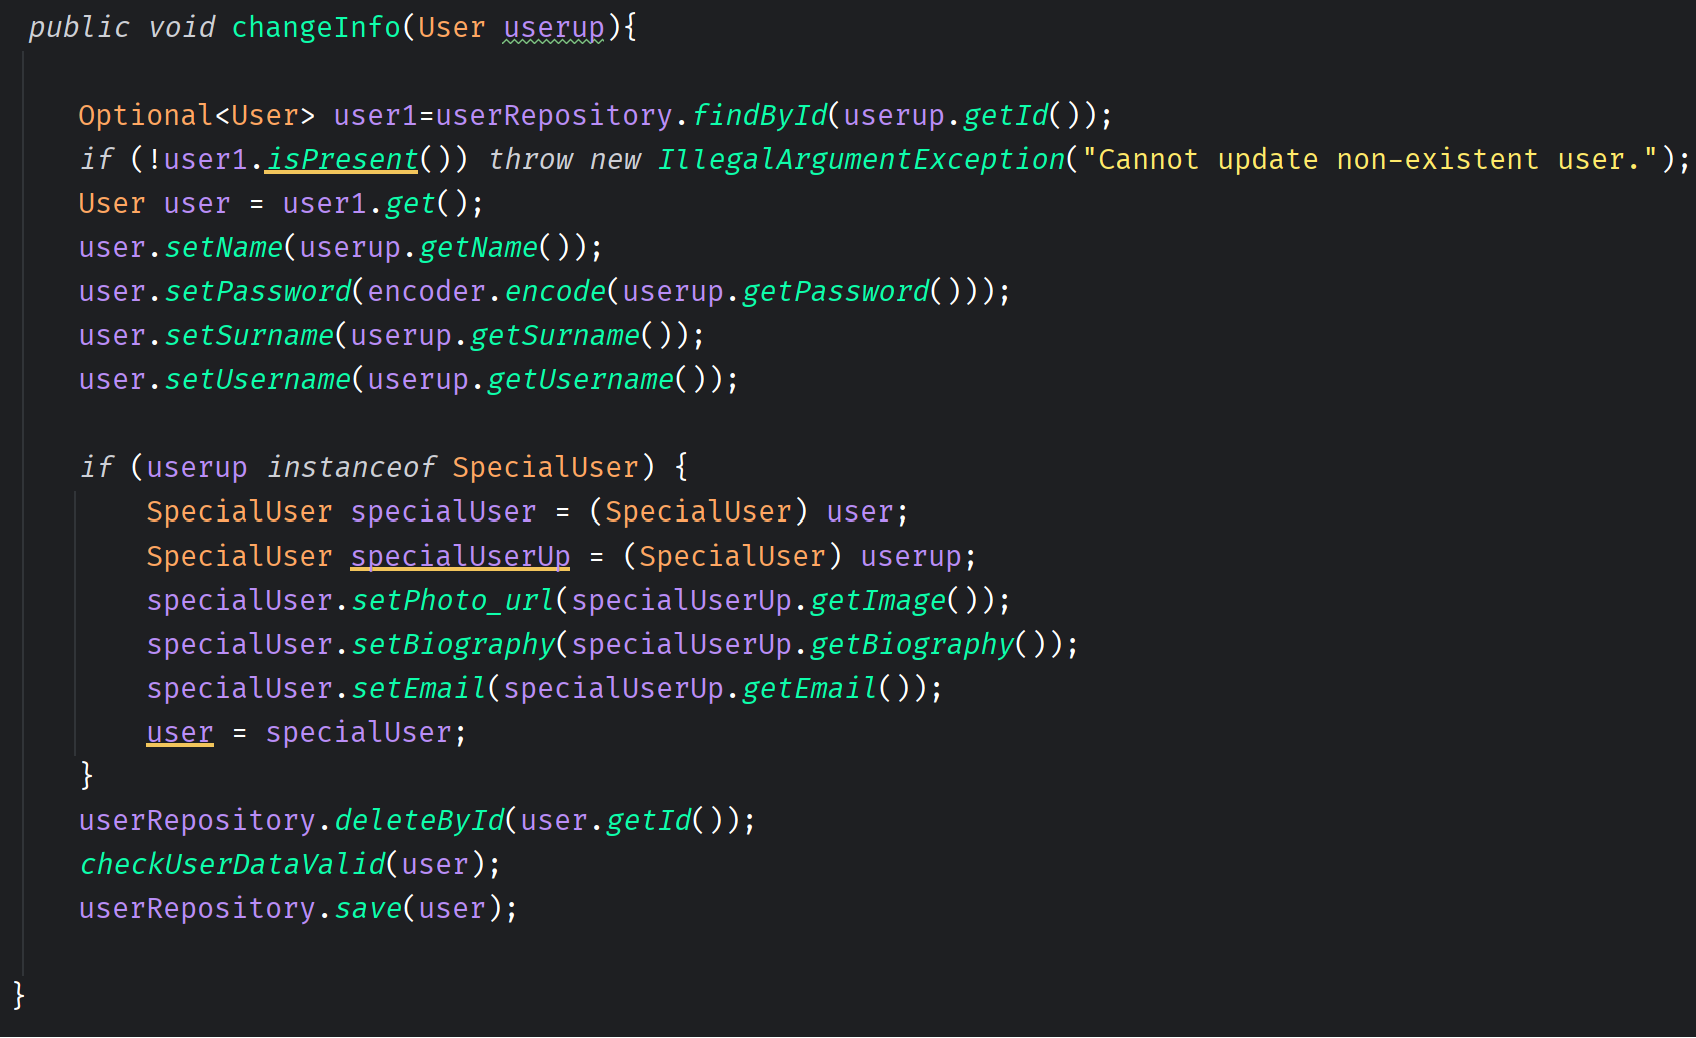
\includegraphics[scale=0.4]{slike/changeInfo.PNG} %veličina slike u odnosu na originalnu datoteku i pozicija slike
			\centering
			\caption{Metoda "changeInfo" klase UserService}
			\label{Metoda "changeInfo" klase UserService}
		\end{figure}
		
			\begin{figure}[H]
			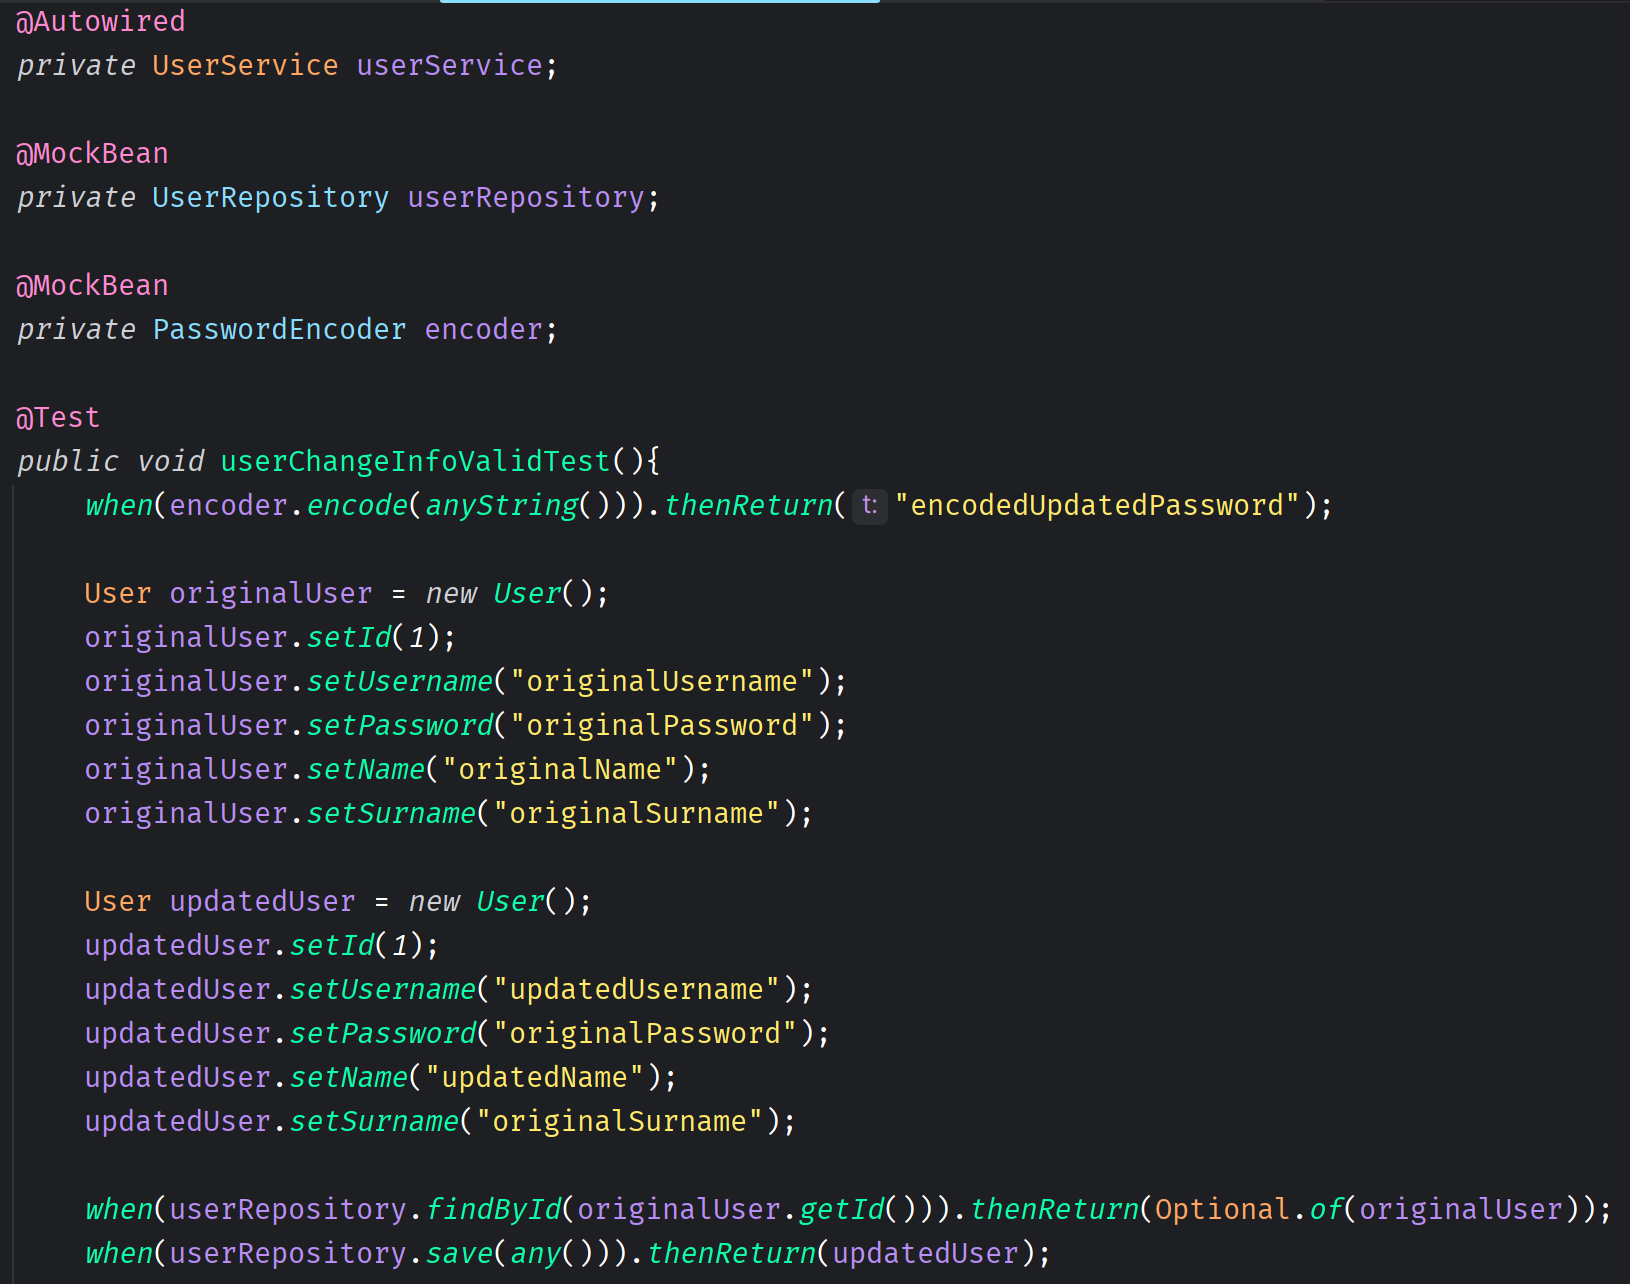
\includegraphics[scale=0.4]{slike/userChangeInfoValidTest1.PNG} %veličina slike u odnosu na originalnu datoteku i pozicija slike
			\centering
			\caption{Test uspješne promjene podataka korisnika u bazi, 1. dio}
			\label{Test uspješne promjene podataka korisnika u bazi, 1. dio}
		\end{figure}
		
								\begin{figure}[H]
			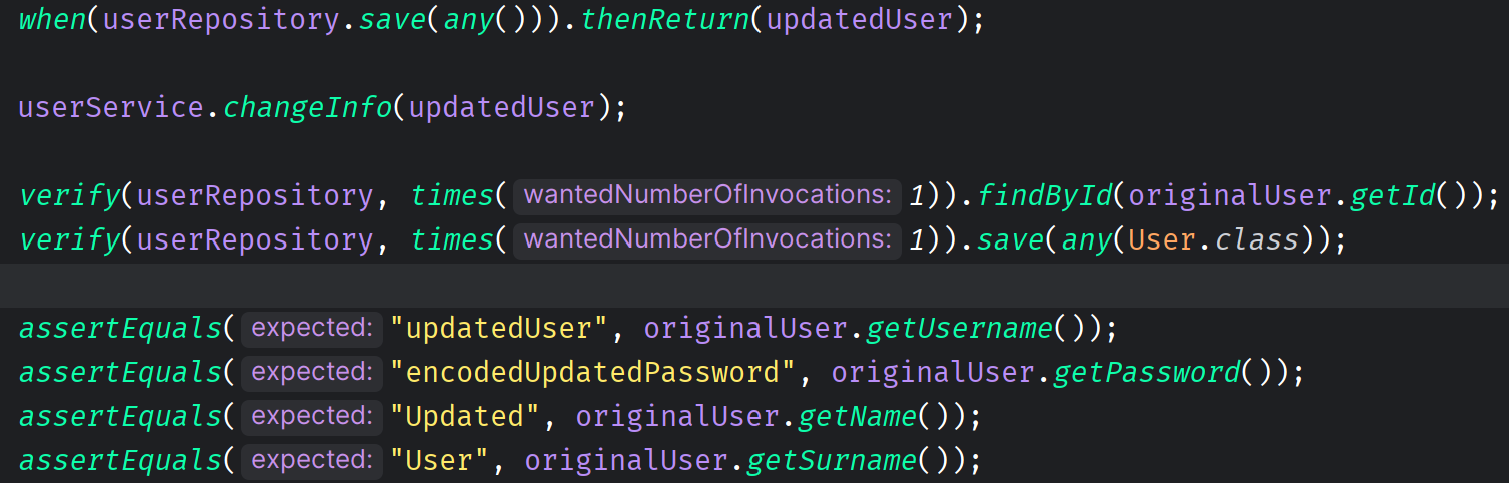
\includegraphics[scale=0.4]{slike/userChangeInfoValidTest2.PNG} %veličina slike u odnosu na originalnu datoteku i pozicija slike
			\centering
			\caption{Test uspješne promjene podataka korisnika u bazi, 2. dio}
			\label{Test uspješne promjene podataka korisnika u bazi, 2. dio}
		\end{figure}
		
		\begin{figure}[H]
			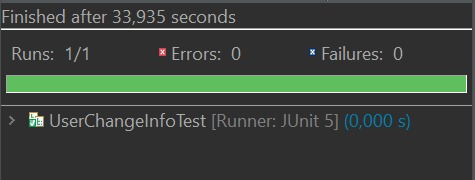
\includegraphics[scale=0.4]{slike/JUnit_change.JPG} %veličina slike u odnosu na originalnu datoteku i pozicija slike
			\centering
			\caption{Potvrda uspješnog izvođenja testova vezanih uz promjenu podataka korisnika}
			\label{Potvrda uspješnog izvođenja testova vezanih uz promjenu podataka korisnika}
		\end{figure}
		
		
			
		\textbf{Test 7: Uspješno dohvaćanje recepata po korisničkom imenu autora recepata}
		
		Provedeno je testiranje uspješnog dohvaćanja recepata po korisničkom imenu autora recepata. Dohvaćanje recepata je uspješno ako dohvaćeni set recepata kojima je autor stvoreni korisnik nije null vrijednost te ako su očekivani set recepata i dohvaćeni set recepata jednaki. Na slikama ispod prikazani su test uspješnog dohvaćanja recepata po korisničkom imenu autora recepata te metoda "getRecipesByUsername" klase RecipeService.
		
		\begin{figure}[H]
			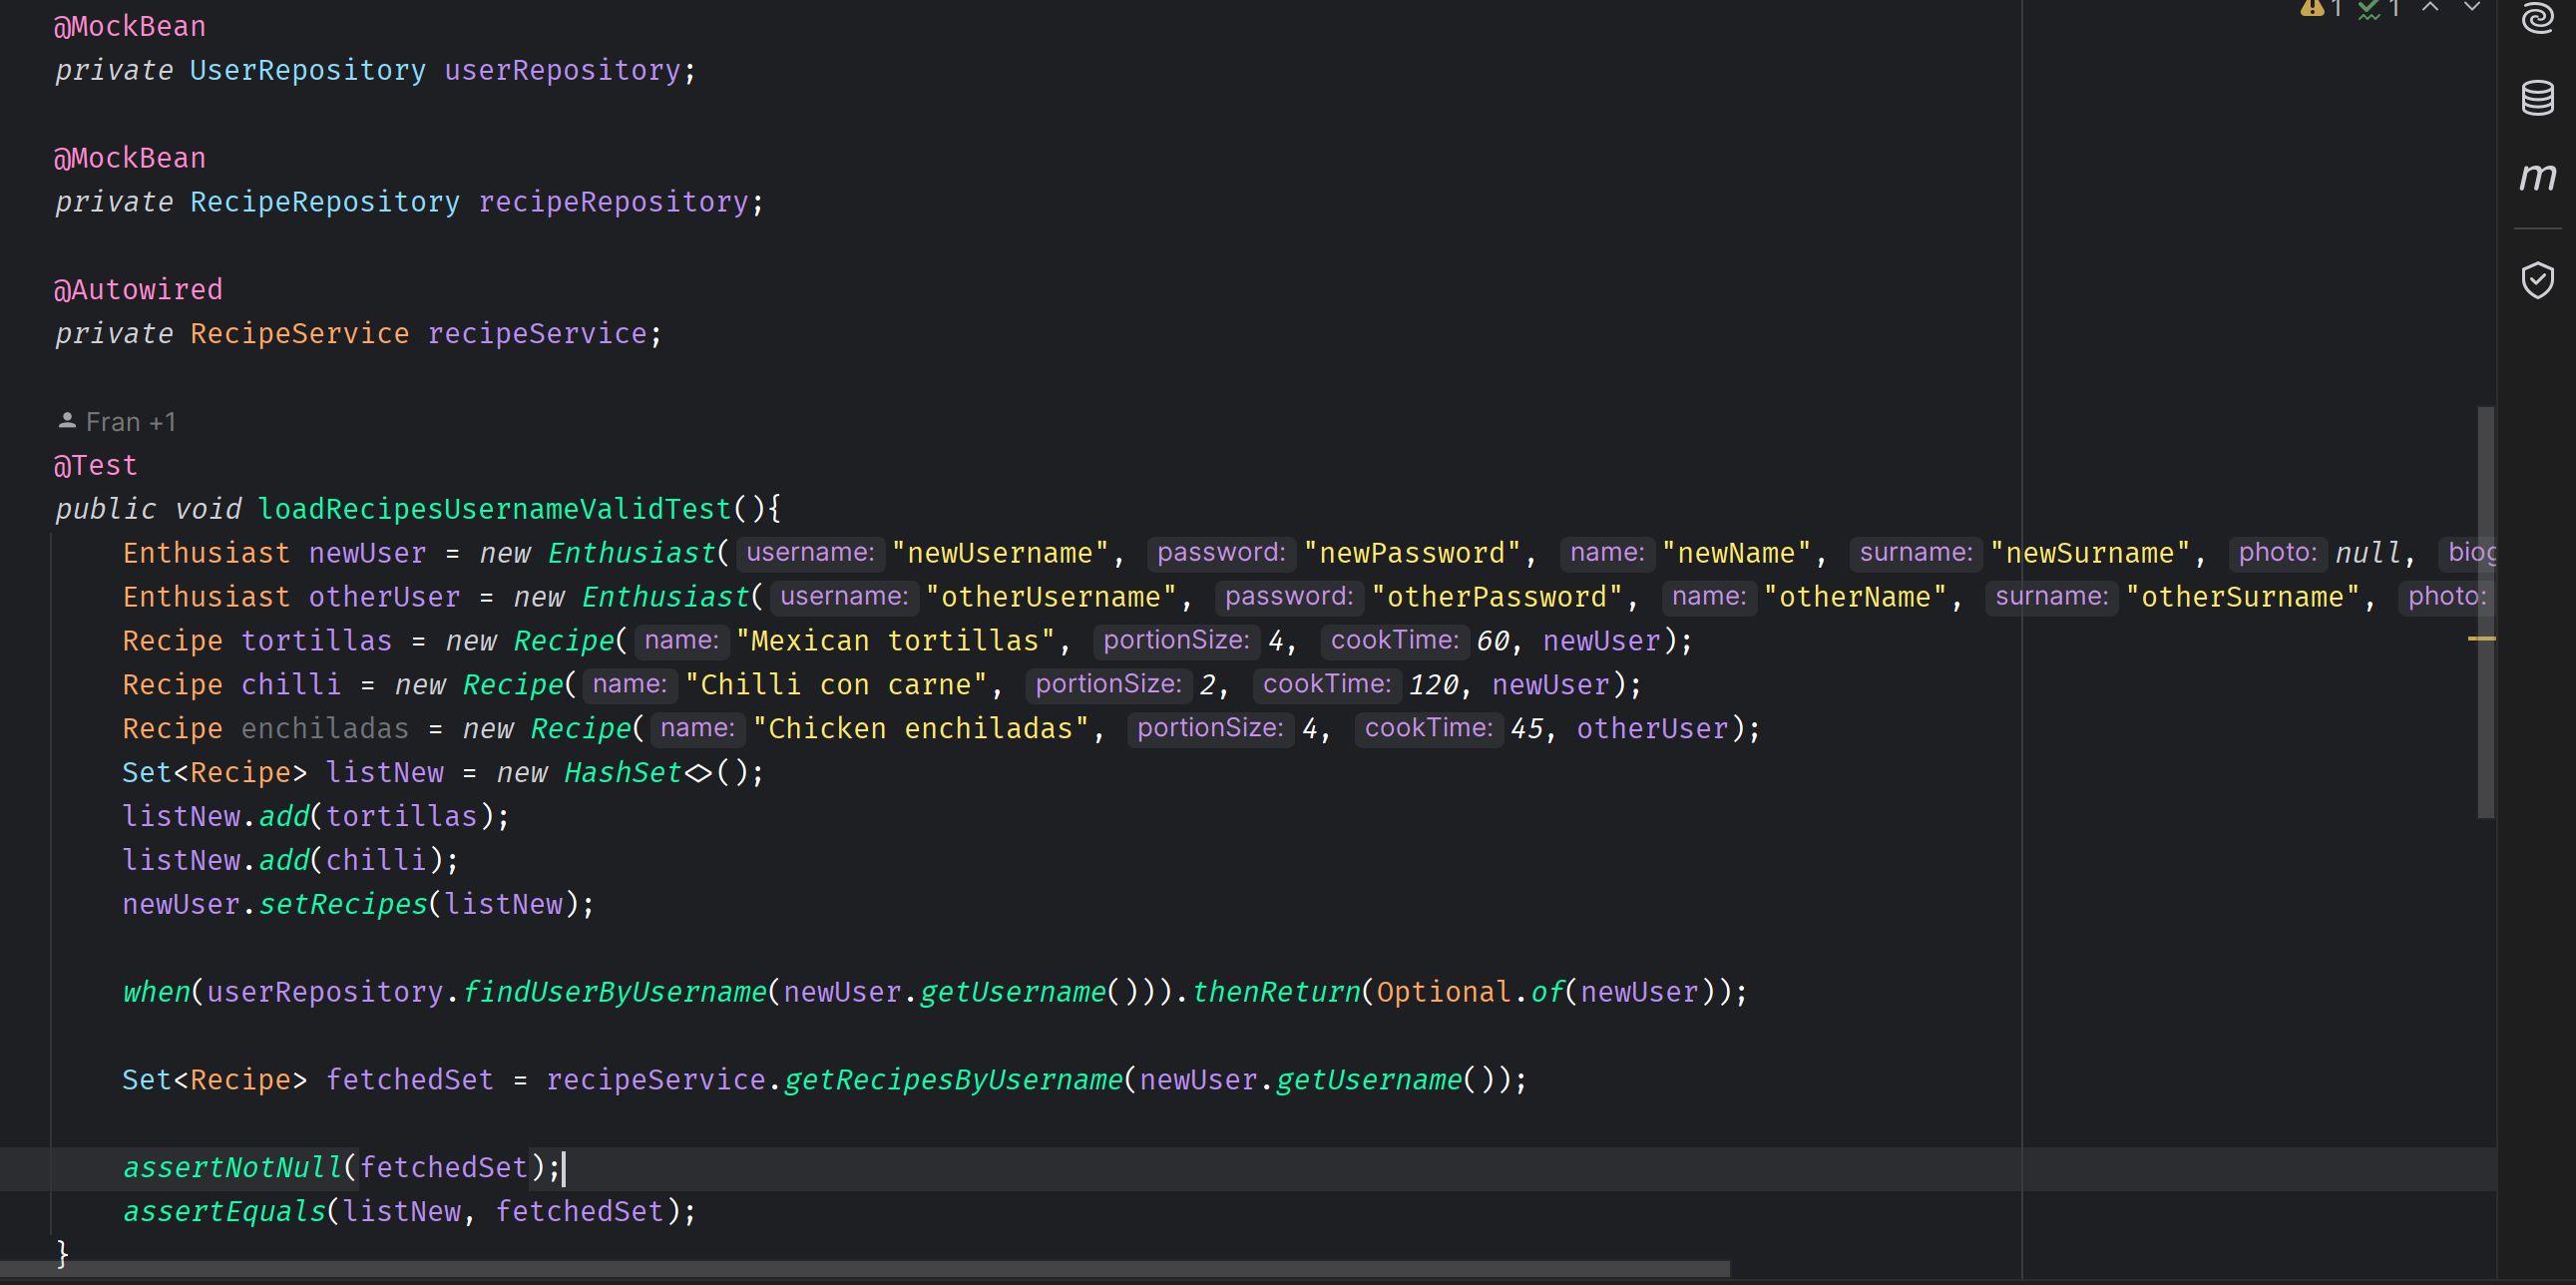
\includegraphics[scale=0.4]{slike/loadRecipesUsernameValidTest.PNG} %veličina slike u odnosu na originalnu datoteku i pozicija slike
			\centering
			\caption{Test uspješnog dohvaćanja recepata po korisničkom imenu}
			\label{Test uspješnog dohvaćanja recepata po korisničkom imenu}
		\end{figure}
		
				\begin{figure}[H]
			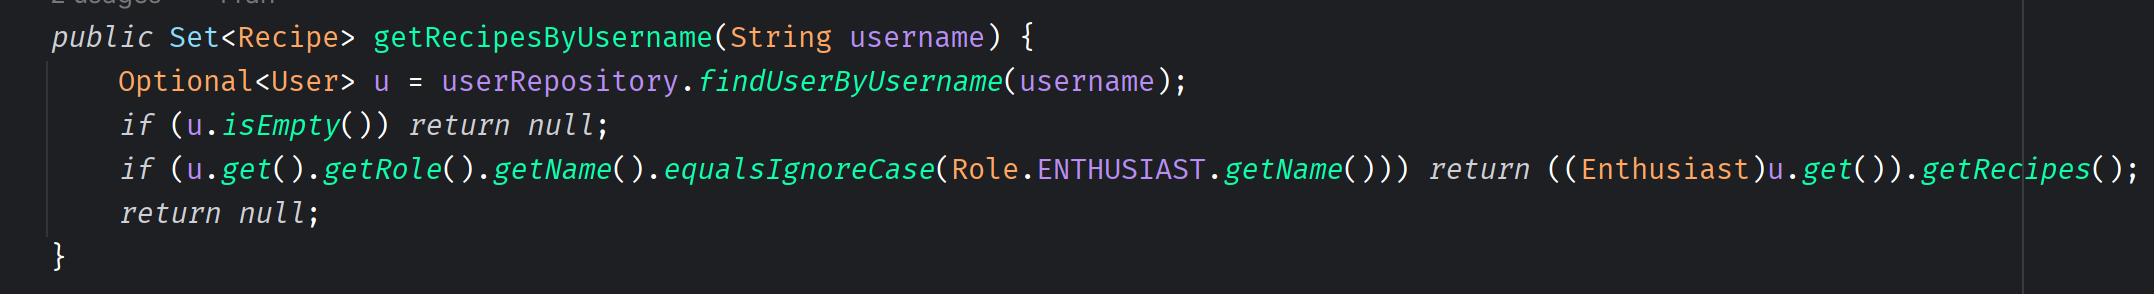
\includegraphics[scale=0.4]{slike/getRecipesByUsername.PNG} %veličina slike u odnosu na originalnu datoteku i pozicija slike
			\centering
			\caption{Metoda "getRecipesByUsername" klase RecipeService}
			\label{Metoda "getRecipesByUsername" klase RecipeService}
		\end{figure}
		
		\textbf{Test 8: Uspješno dohvaćanje recepata po kategoriji recepta}
		
		Provedeno je testiranje uspješnog dohvaćanja recepata po kategoriji recepta. Dohvaćanje recepata je uspješno ako dohvaćeni set recepata iz oponašanog repozitorija recepata s određenom kategorijom nije null vrijednost te ako su očekivani set recepata i dohvaćeni set recepata jednaki. Na slikama ispod prikazani su test uspješnog dohvaćanja recepata po kategoriji te metoda "getRecipesByCategory" klase RecipeService.
		
				\begin{figure}[H]
			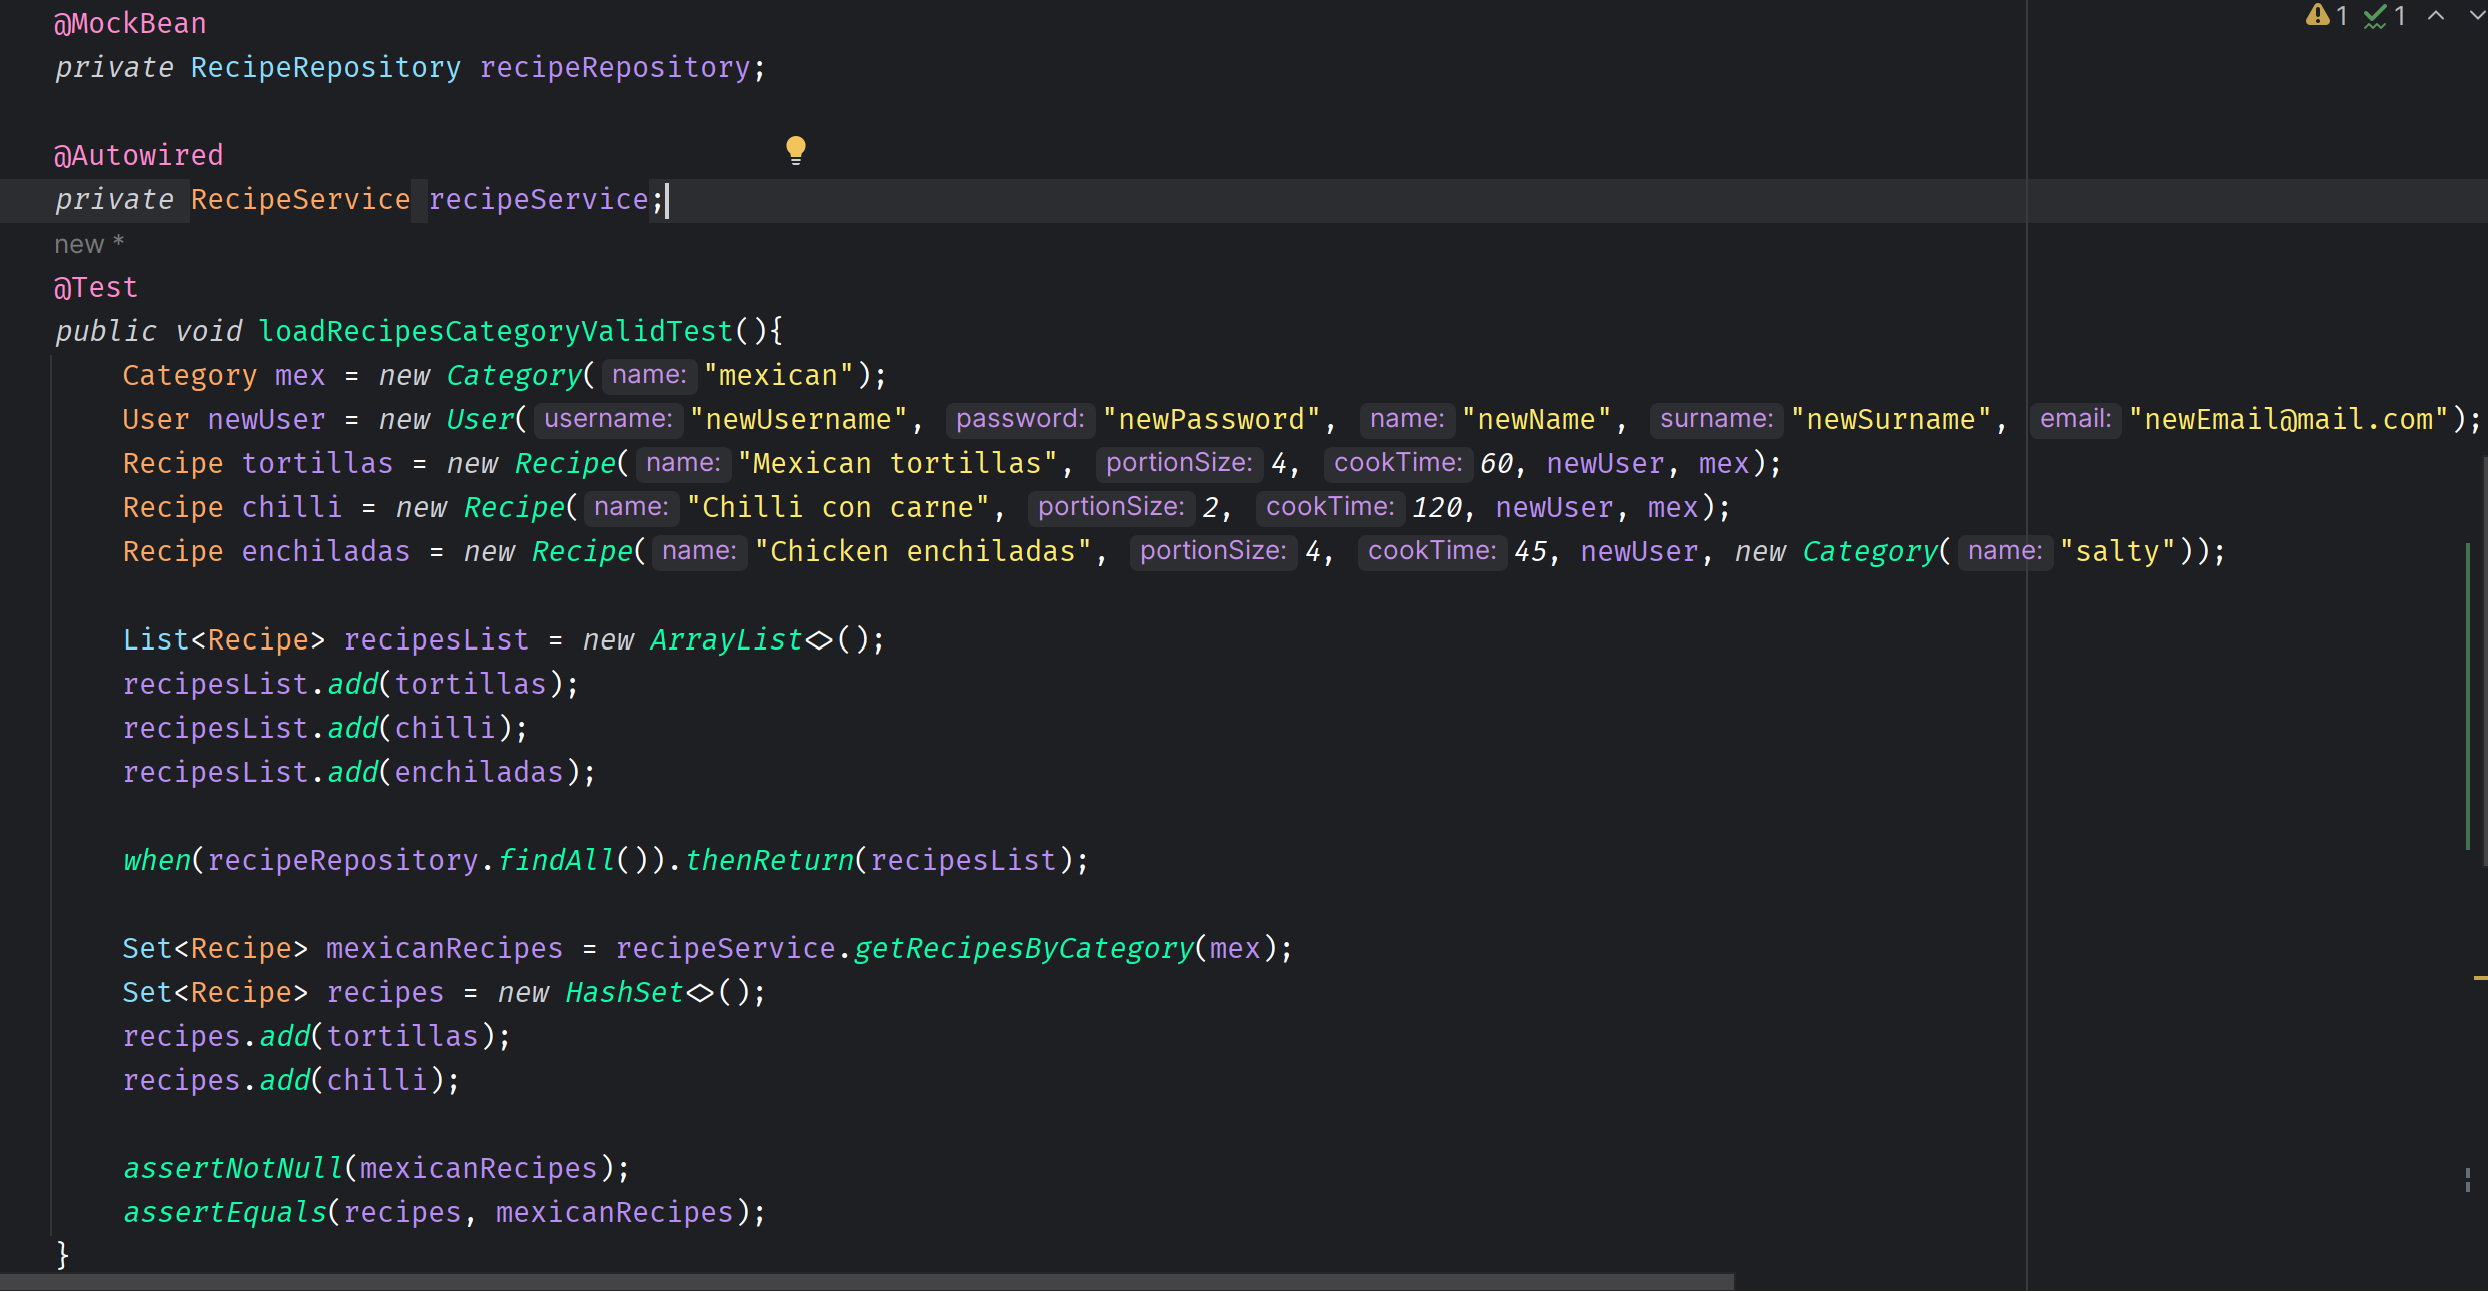
\includegraphics[scale=0.4]{slike/loadRecipesCategoryValidTest.PNG} %veličina slike u odnosu na originalnu datoteku i pozicija slike
			\centering
			\caption{Test uspješnog dohvaćanja recepata po kategoriji}
			\label{Test uspješnog dohvaćanja recepata po kategoriji}
		\end{figure}
		
			\begin{figure}[H]
			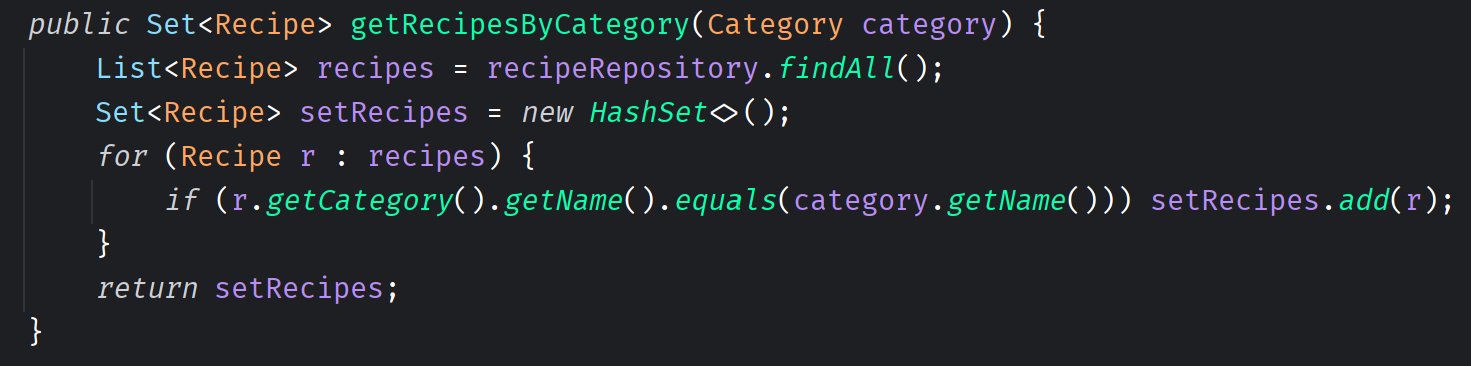
\includegraphics[scale=0.4]{slike/getRecipesByCategory.PNG} %veličina slike u odnosu na originalnu datoteku i pozicija slike
			\centering
			\caption{Metoda "getRecipesByCategory" klase RecipeService}
			\label{Metoda "getRecipesByCategory" klase RecipeService}
		\end{figure}
		
		Na slici ispod prikazana je potvrda uspješnosti izvođenja testova o dohvaćanju recepata na temelju korisničkog imena/kategorije.
		
		\begin{figure}[H]
			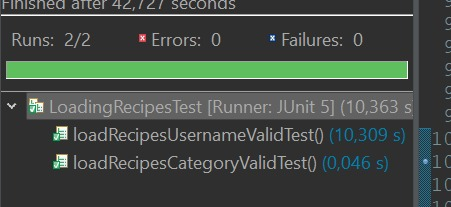
\includegraphics[scale=0.4]{slike/JUnit_loadRecipes.JPG} %veličina slike u odnosu na originalnu datoteku i pozicija slike
			\centering
			\caption{Potvrda uspješnog izvođenja testova vezanih uz dohvaćanje recepata}
			\label{Potvrda uspješnog izvođenja testova vezanih uz dohvaćanje recepata}
		\end{figure}
		
		
		
		

		
		

















			
			
			
			\subsection{Ispitivanje sustava}
			
			 \textit{Potrebno je provesti i opisati ispitivanje sustava koristeći radni okvir Selenium\footnote{\url{https://www.seleniumhq.org/}}. Razraditi \textbf{minimalno 4 ispitna slučaja} u kojima će se ispitati redovni slučajevi, rubni uvjeti te poziv funkcionalnosti koja nije implementirana/izaziva pogrešku kako bi se vidjelo na koji način sustav reagira kada nešto nije u potpunosti ostvareno. Ispitni slučaj se treba sastojati od ulaza (npr. korisničko ime i lozinka), očekivanog izlaza ili rezultata, koraka ispitivanja i dobivenog izlaza ili rezultata.\\ }
			 
			 \textit{Izradu ispitnih slučajeva pomoću radnog okvira Selenium moguće je provesti pomoću jednog od sljedeća dva alata:}
			 \begin{itemize}
			 	\item \textit{dodatak za preglednik \textbf{Selenium IDE} - snimanje korisnikovih akcija radi automatskog ponavljanja ispita	}
			 	\item \textit{\textbf{Selenium WebDriver} - podrška za pisanje ispita u jezicima Java, C\#, PHP koristeći posebno programsko sučelje.}
			 \end{itemize}
		 	\textit{Detalji o korištenju alata Selenium bit će prikazani na posebnom predavanju tijekom semestra.}
			
			\eject 
		
		
		\section{Dijagram razmještaja}
			
		
		Na slici 5.1 prikazan je dijagram razmještaja. Dijagrami razmještaja prikazuju fizičku arhitekturu programskog sustava, prikazujući razmještaj programskih artefakata na sklopovskim čvorovima ili virtualnim okruženjima. Glavna svrha dijagrama razmještaja u programskom inženjerstvu je pružiti razumijevanje arhitekture razmještaja sustava.
		
		Naš dijagram razmještaja sastoji se od dvije glavne komponente: računalo korisnika i poslužiteljsko računalo. Na računalu korisnika, on putem web preglednika pristupa aplikaciji KuhajIT. Komunikacija između računala korisnika i poslužiteljskog računala uspostavlja se i odvija pomoću protokola HTTP. Unutar poslužiteljskog računala razlikujemo dvije podkomponente: web poslužitelj i poslužitelj baze podataka.
		
					\begin{figure}[H]
			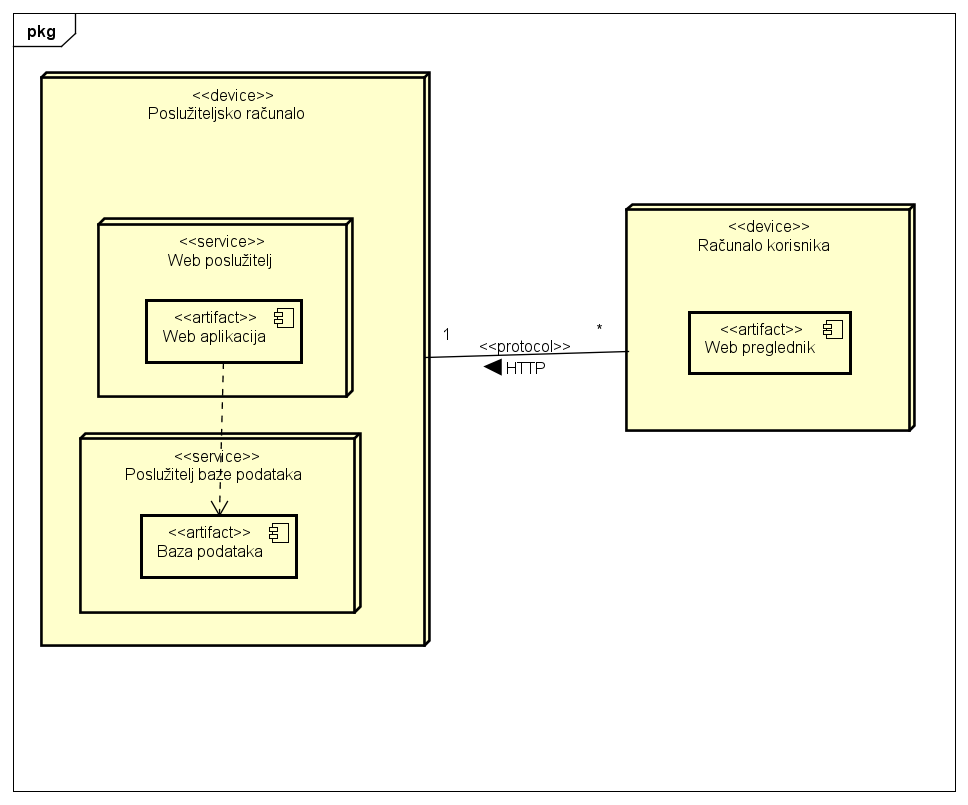
\includegraphics[scale=0.4]{dijagrami/UML_dijagram_razmjestaja.PNG} %veličina slike u odnosu na originalnu datoteku i pozicija slike
			\centering
			\caption{Dijagram razmještaja}
			\label{Dijagram razmještaja}
		\end{figure}
		
		

			\eject 
		
		\section{Upute za puštanje u pogon}
		Naša KuhajIT web-aplikacija, razvijena u okviru ovog projekta, puštena je u pogon putem web platforme  \textcolor{blue}{\underline{\href{https://render.com/}{\textcolor{blue}{Render}}}}\footnote{\url{https://render.com/}}. Render je platforma koja pruža usluge za deploy, hosting i skaliranje web aplikacija, servisa i web stranica. Ističe se jednostavnošću upotrebe, brzim implementacijama i podrškom za različite jezike i okvire, i upravo smo ju zbog tog razloga i odabrali za tzv. deploy. Na Render-u je postavljen Spring Boot poslužitelj, kojega smo spremili u Docker kontejner, a koji odgovara na upite korisnika, statička stranica, koja služi za prikaz React web aplikacije te PostgreSQL baza podataka. Ispod su priložene dvije slike komponenata postavljenih na Render.
		
		
			\begin{figure}[H]
			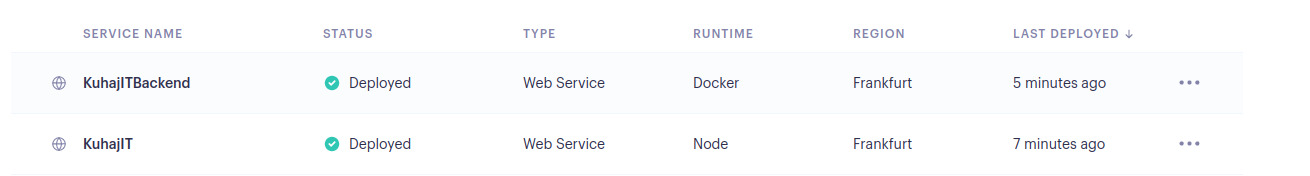
\includegraphics[scale=0.3]{slike/Render_OVERVIEW.JPG} %veličina slike u odnosu na originalnu datoteku i pozicija slike
			\centering
			\caption{Pregled prenesenih komponenti, frontend i backend}
			\label{Pregled prenesenih komponenti, frontend i backend}
		\end{figure}
		
					\begin{figure}[H]
			
\includegraphics[scale=0.3]{slike/Render_OVERVIEW_DATABASE.JPG} %veličina slike u odnosu na originalnu datoteku i pozicija slike
			\centering
			\caption{Pregled prenesenih komponenti, baza podataka}
			\label{Pregled prenesenih komponenti, baza podataka}
		\end{figure}
		
		
		
		\textbf{Postavljanje Spring Boot poslužitelja} \\
		Dio razloga zbog kojeg smo odabrali baš Render za deploy je jednostavnost postavljanja komponenti na njega. Tako je bilo i s postavljanjem Spring Boot poslužitelja koji komunicira sa React aplikacijom, spremljenom u \textcolor{blue}{\underline{\href{https://docker.com/}{\textcolor{blue}{Docker}}}}\footnote{\url{https://docker.com/}} "kontejner". Korištenje Docker-a nam je uvelike olakšalo cijeli proces deploy-a, jer Docker nudi izolirane okoline, zvane kontejnerima, koje sadrže sve potrebno za pokretanje aplikacije, stoga se nije potrebno oslanjati na ono što je instalirano na Render poslužitelju. Na slici ispod prikazan je kod Dockerfile-a. Dockerfile je dokument koji sadrži sve naredbe koje bi se trebale pozvati u naredbenom retku kako bi se aplikacija ispravno i cjelovito pokrenula.
		
		\begin{figure}[H]
			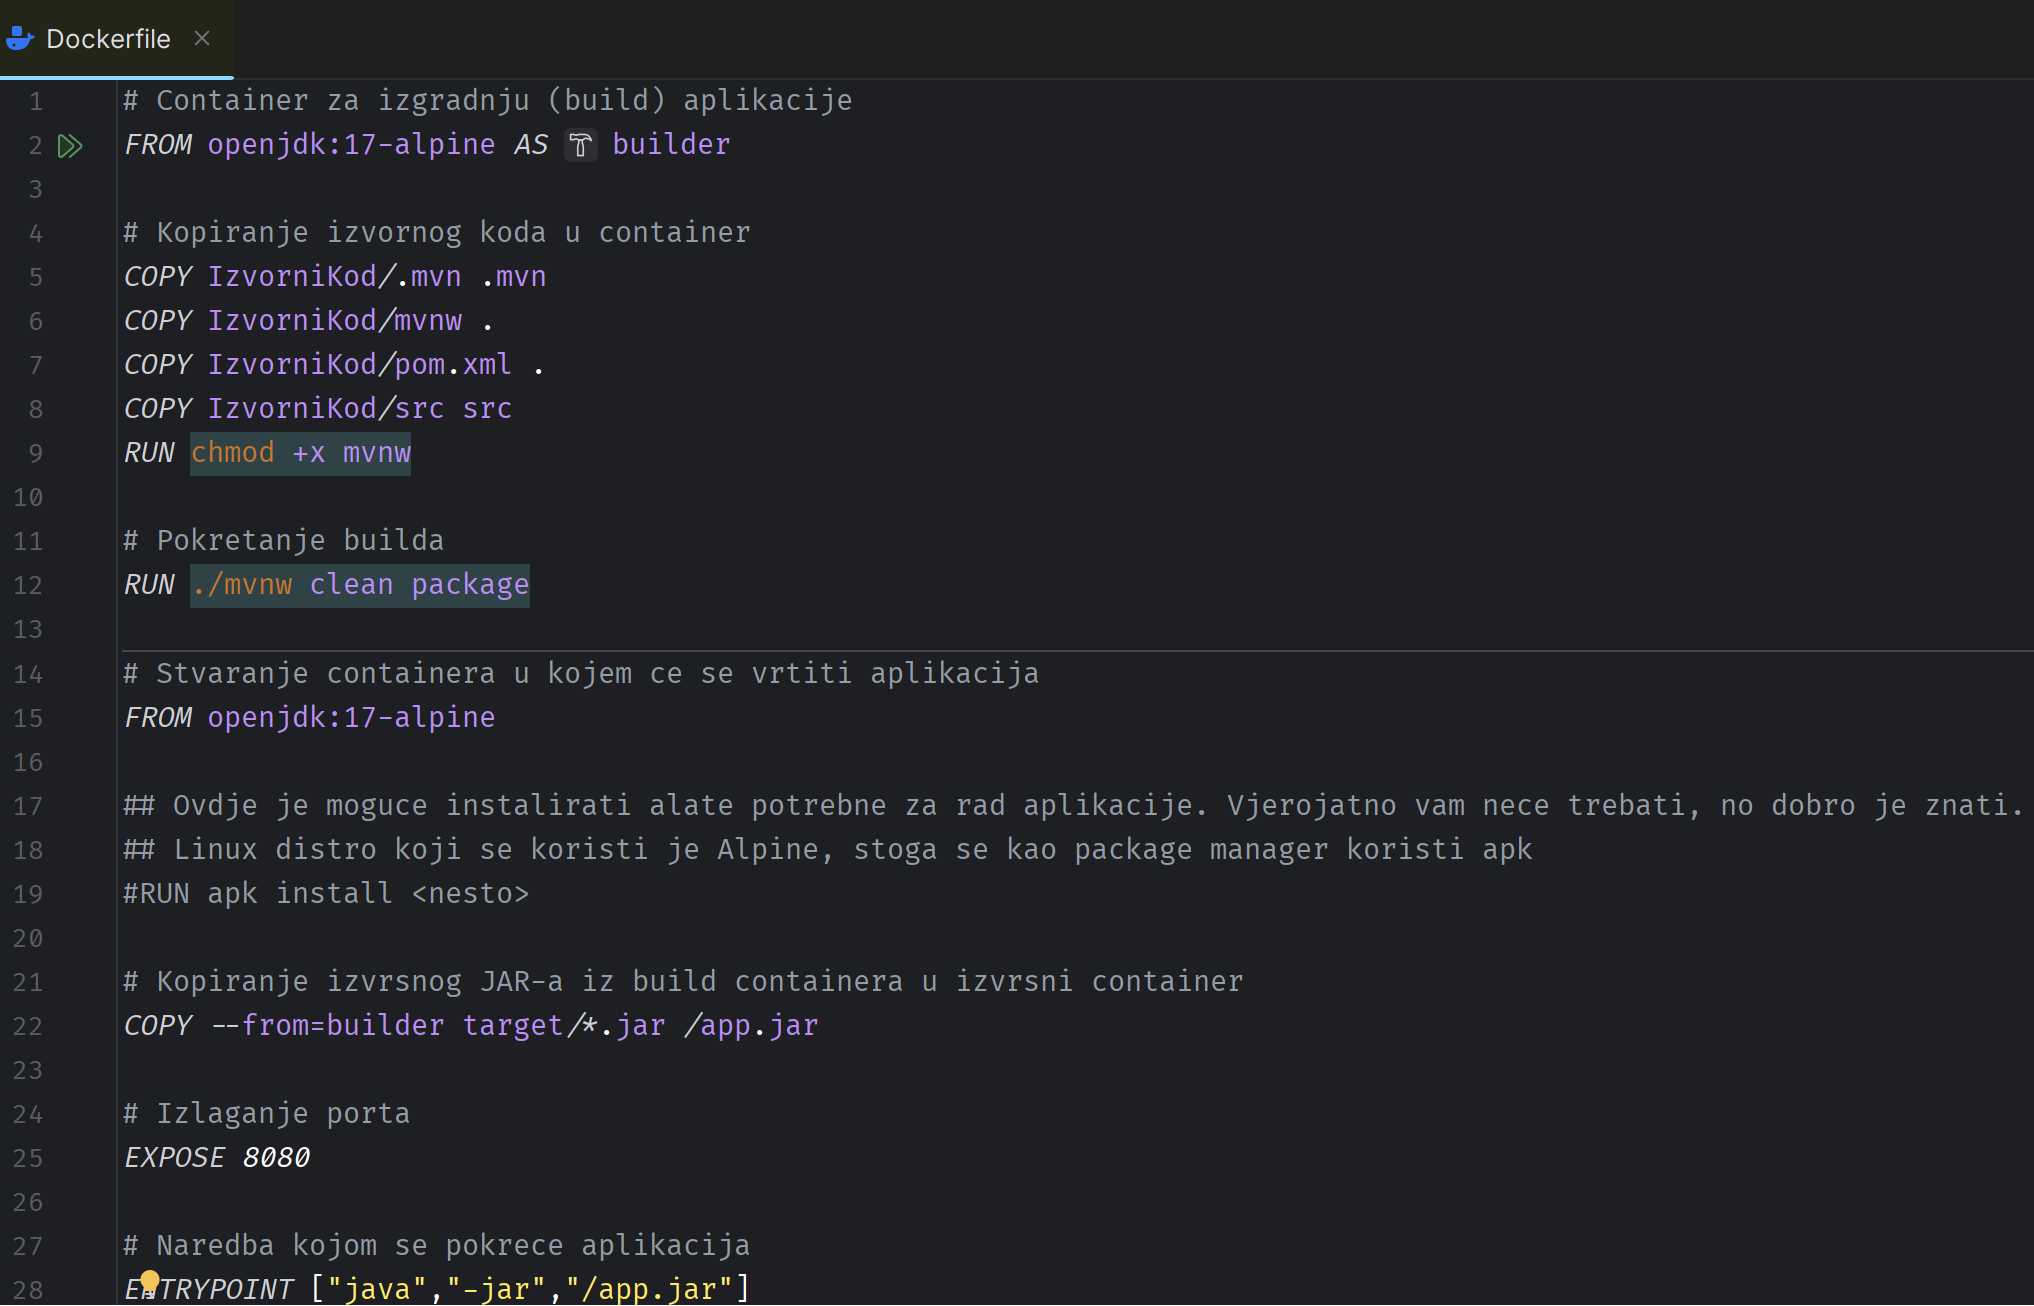
\includegraphics[scale=0.4]{slike/Dockerfile.PNG} %veličina slike u odnosu na originalnu datoteku i pozicija slike
			\centering
			\caption{Dockerfile}
			\label{Dockerfile}
		\end{figure}
		
		
Na početku, potrebno je u gornjem desnom kutu web platforme Render odabrati opciju New, kako je prikazano na slici ispod.
		
			\begin{figure}[H]
			
\includegraphics[scale=0.4]{slike/Render_NEW.PNG} %veličina slike u odnosu na originalnu datoteku i pozicija slike
			\centering
			\caption{Dodavanje nove komponente}
			\label{Dodavanje nove komponente}
		\end{figure}
		
		Zatim, u izborniku koji se prikaže, potrebno je odabrati opciju Web Service, kako je prikazano na slici ispod.
					\begin{figure}[H]
			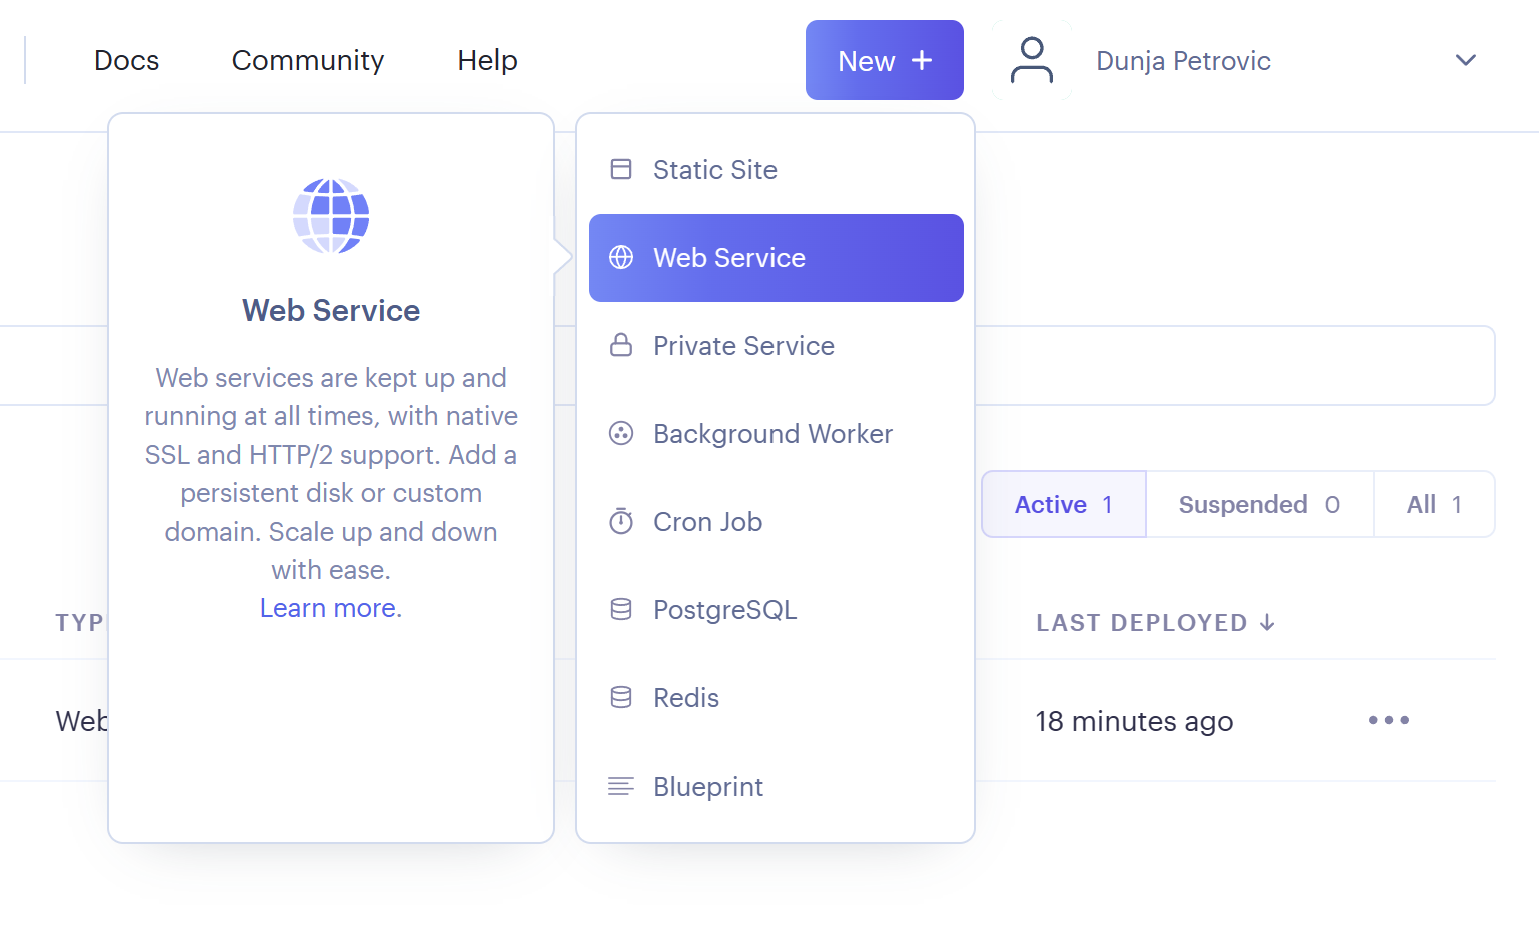
\includegraphics[scale=0.4]{slike/Render_WEB_SERVICE.PNG} %veličina slike u odnosu na originalnu datoteku i pozicija slike
			\centering
			\caption{Odabir opcije Web Service}
			\label{Odabir opcije Web Service}
		\end{figure}
		
		Kada nam se otvori stranica za dodavanje nove komponente tipa "Web Service", nudi nam se opcija odabira GitHub repozitorija iz koje želimo dodati komponentu, koju je potrebno i označiti, kako je prikazano na slici ispod.
		
			\begin{figure}[H]
			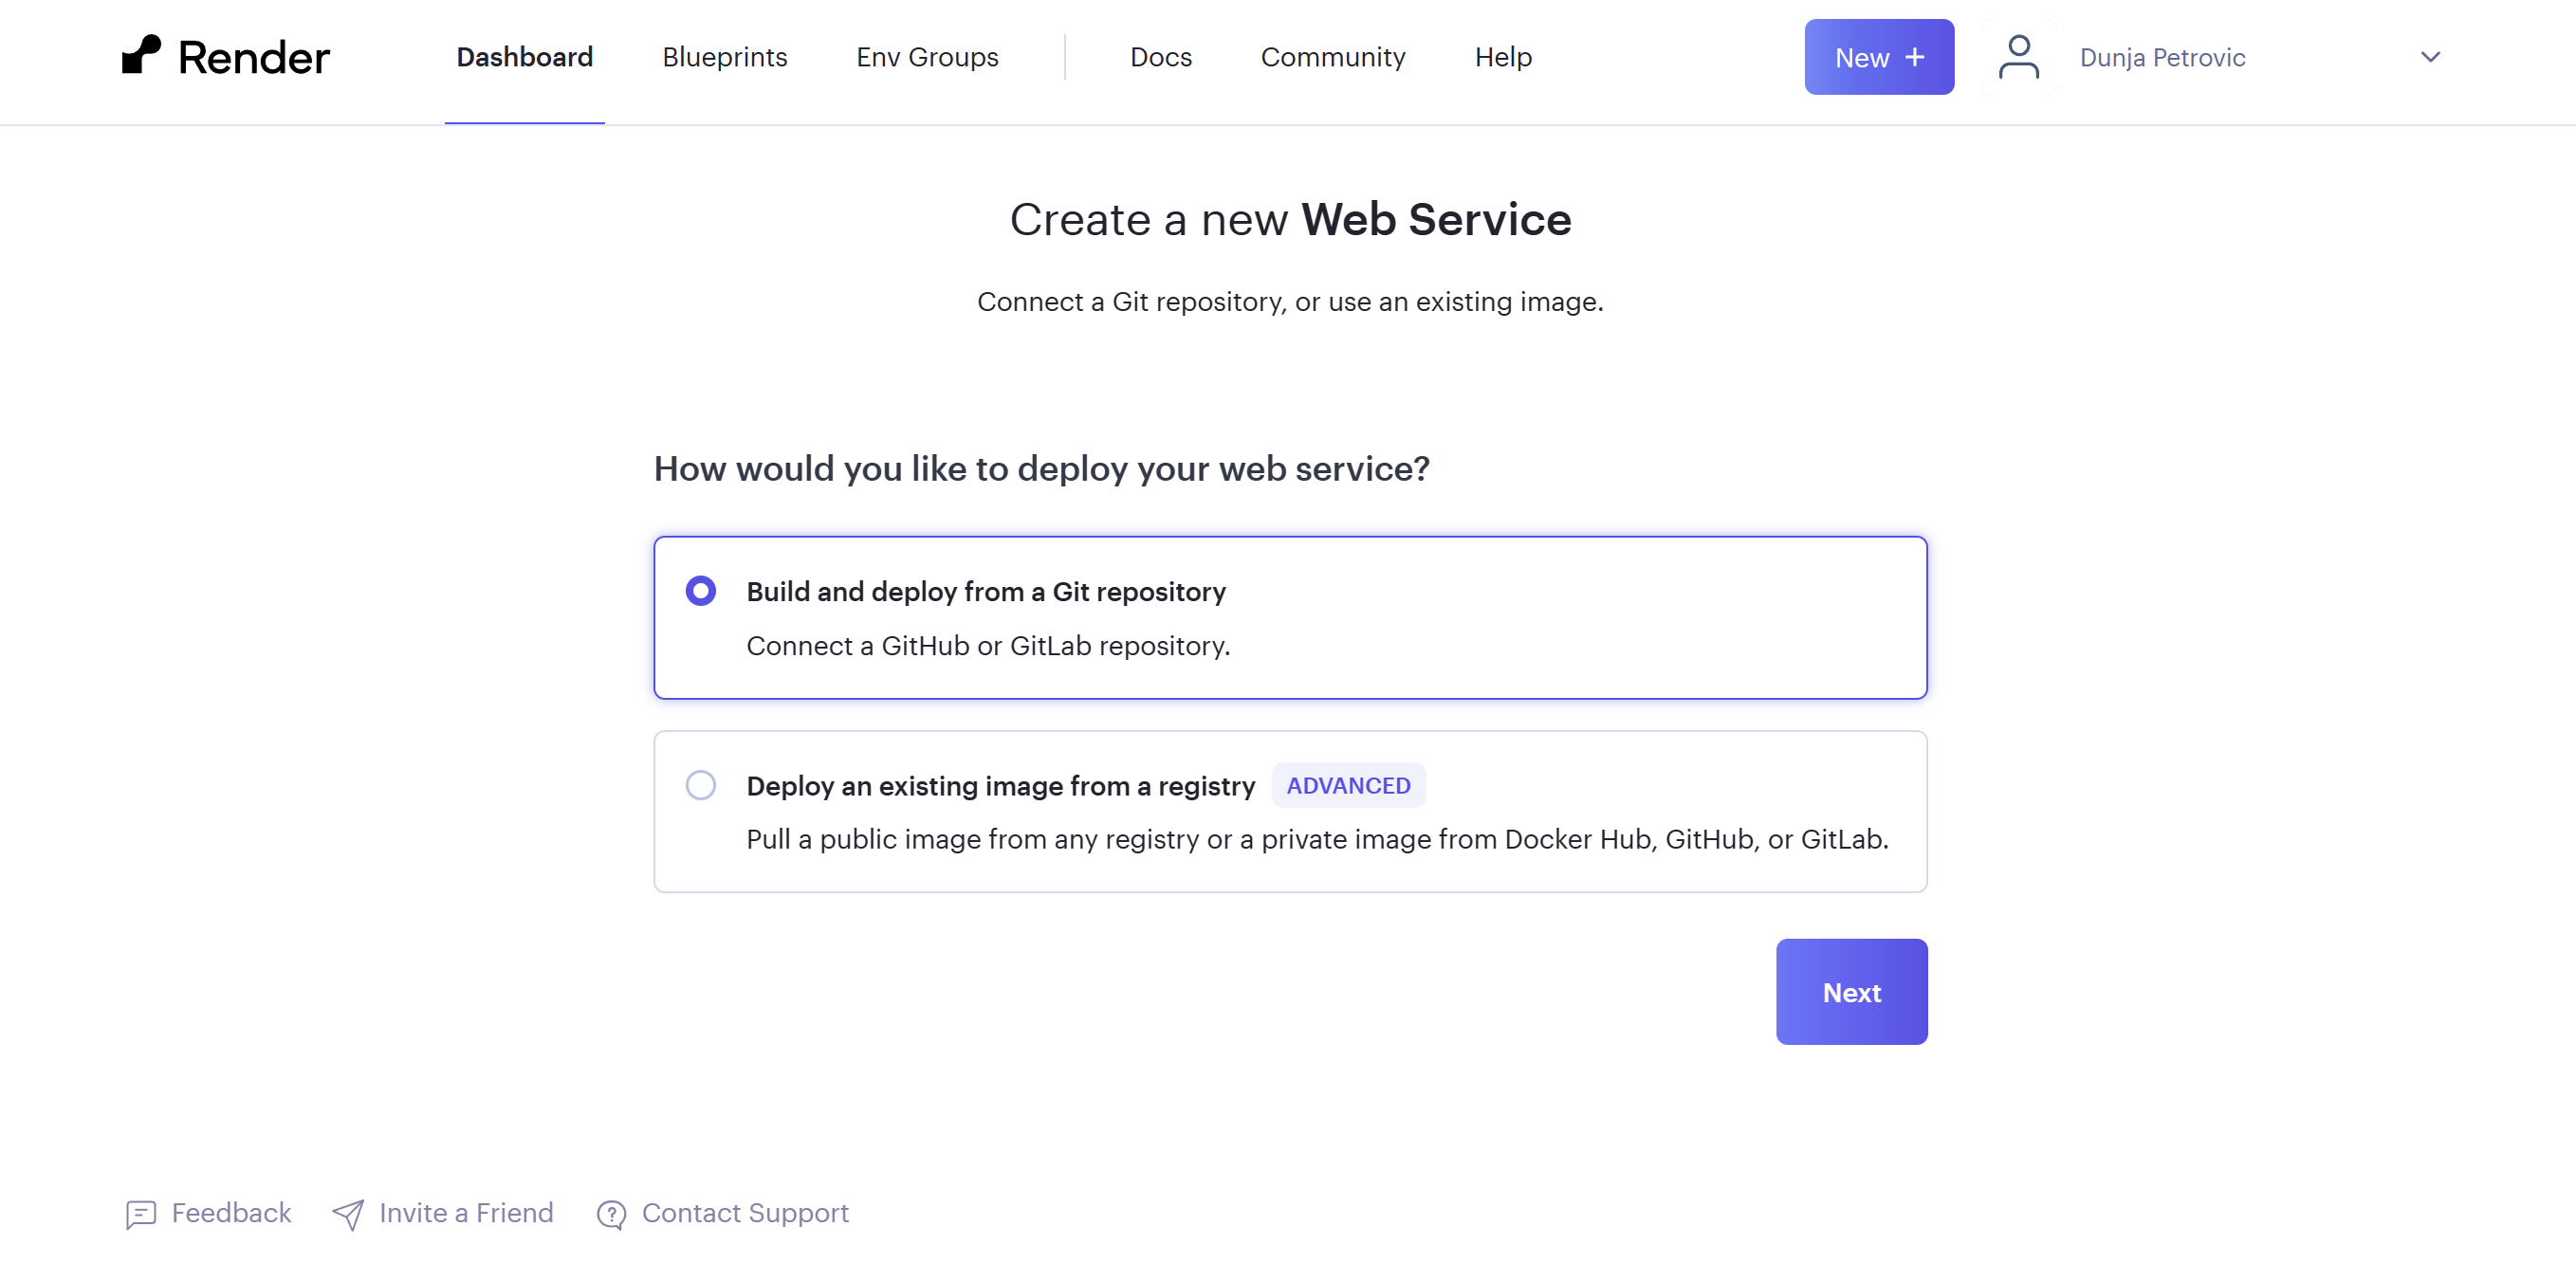
\includegraphics[scale=0.4]{slike/Render_ODABIR_OPCIJE.PNG} %veličina slike u odnosu na originalnu datoteku i pozicija slike
			\centering
			\caption{Odabir opcije dodavanja iz postojećeg GitHub repozitorija}
			\label{Odabir opcije dodavanja iz postojećeg GitHub repozitorija}
		\end{figure}
		
	    Nakon povezivanja Render računa s GitHub računom, slijedi odabir repozitorija, kako je prikazano na slici ispod. Mi smo odabrali repozitorij ljubo9/30bodova.
	    
	    	\begin{figure}[H]
			\includegraphics[scale=0.4]{slike/Render_ODABIR_REPOZITORIJA.PNG} %veličina slike u odnosu na originalnu datoteku i pozicija slike
			\centering
			\caption{Odabir repozitorija}
			\label{Odabir repozitorija}
		\end{figure}
		
		Odabir repozitorija slijedi podešavanje svih potrebnih opcija kako bi se Spring Boot poslužitelj ispravno pokrenuo. Na slici ispod prikazane su postavke koje je potrebno postaviti za ispravan rad poslužitelja.
		
		\begin{figure}[H]
			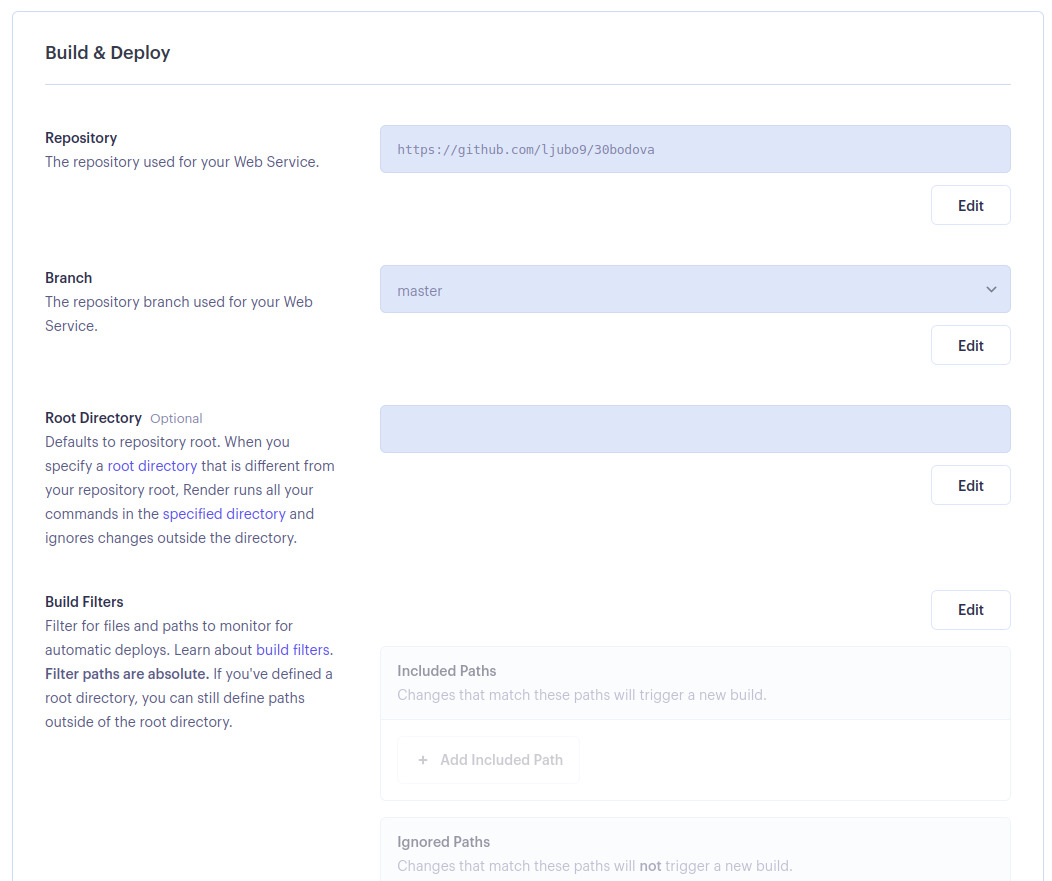
\includegraphics[scale=0.4]{slike/Render_BACKEND_1.JPG} %veličina slike u odnosu na originalnu datoteku i pozicija slike
			\centering
			\caption{Postavke za postavljanje Spring Boot poslužitelja, 1. dio}
			\label{Postavke za postavljanje Spring Boot poslužitelja, 1. dio}
		\end{figure}
		
		Na gornjoj je slici još jednom vidljiv odabrani repozitorij, odabrana grana (mi smo odabrali granu "master") i korijenski direktorij (nama to nije bilo važno pa smo ga ostavili praznog).
		
		Na slici ispod može se vidjeti drugi dio potrebnih postavki za postavljanje Spring Boot poslužitelja.
		
				\begin{figure}[H]
			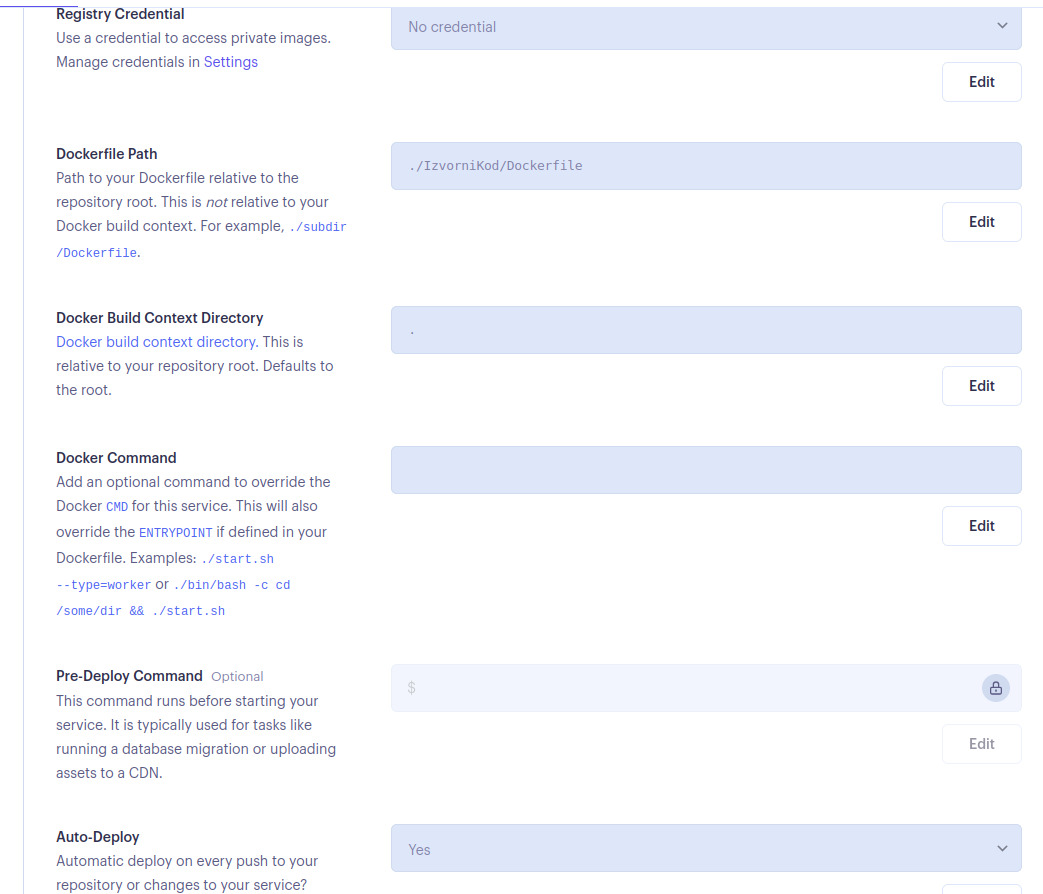
\includegraphics[scale=0.4]{slike/Render_BACKEND_2.JPG} %veličina slike u odnosu na originalnu datoteku i pozicija slike
			\centering
			\caption{Postavke za postavljanje Spring poslužitelja, 2. dio}
			\label{Postavke za postavljanje Spring poslužitelja, 2. dio}
		\end{figure}
		
		Ono što je bilo važno podesiti je bila lokacija Dockerfile-a, koju smo mi podesili na ./IzvorniKod/Dockerfile. Usto, označili smo i opciju "Auto-Deploy" s "Yes" , tako da se svaki put kada se neka nova izmjena napravi u kodu, Spring Boot poslužitelj se iznova "deploy-a". Time je deploy Spring Boot poslužitelja priveden kraju. \\
		
	\textbf{Postavljanje React web aplikacije} \\
	Kao i postavljanje Spring Boot poslužitelja, postavljanje React web aplikacije na Render je izrazito jednostavno. Svi koraci do podešavanja postavki za ispravan rad React web aplikacije jednaki su kao za postavljanje Spring Boot poslužitelja: dodavanje novog "web service-a", odabir opcije spajanja s GitHub repozitorijem, spajanje sa željenim GitHub računom te odabir GitHub repozitorija u kojem se nalazi projekt.
	
	Ono što se razlikuje je podešavanje ispravnih postavki za pokretanje React web aplikacije. Na slici ispod prikazane su potrebne postavke.
	
		\begin{figure}[H]
			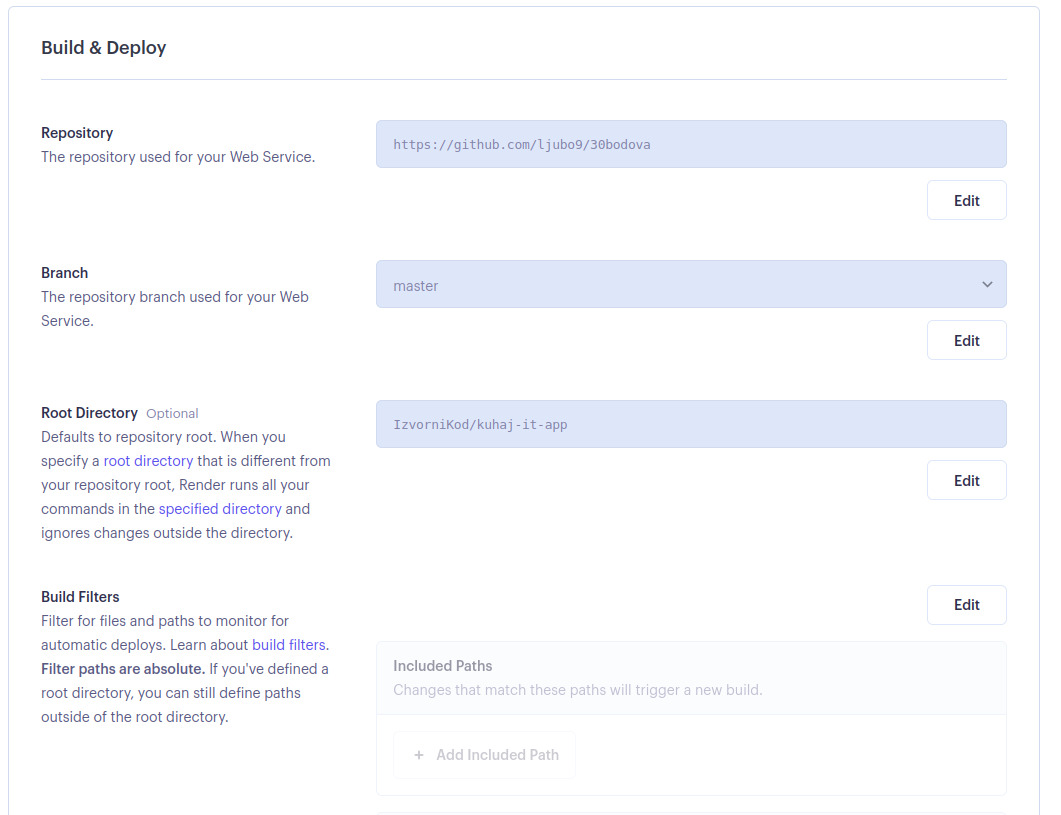
\includegraphics[scale=0.4]{slike/Render_FRONTEND_1.JPG} %veličina slike u odnosu na originalnu datoteku i pozicija slike
			\centering
			\caption{Postavke za postavljanje React web aplikacije, 1. dio}
			\label{Postavke za postavljanje React web aplikacije, 1. dio}
		\end{figure}
		
	Odabrani repozitorij isti je kao za postavljanje Spring Boot poslužitelja, kao i odabrana grana repozitorija.
	Za razliku od postavljanja Spring Boot poslužitelja, ovdje smo za korijenski direktorij odabrali direktorij IzvorniKod/kuhaj-it-app. Drugi dio potrebnih postavki prikazan je na slici ispod.
	
			\begin{figure}[H]
			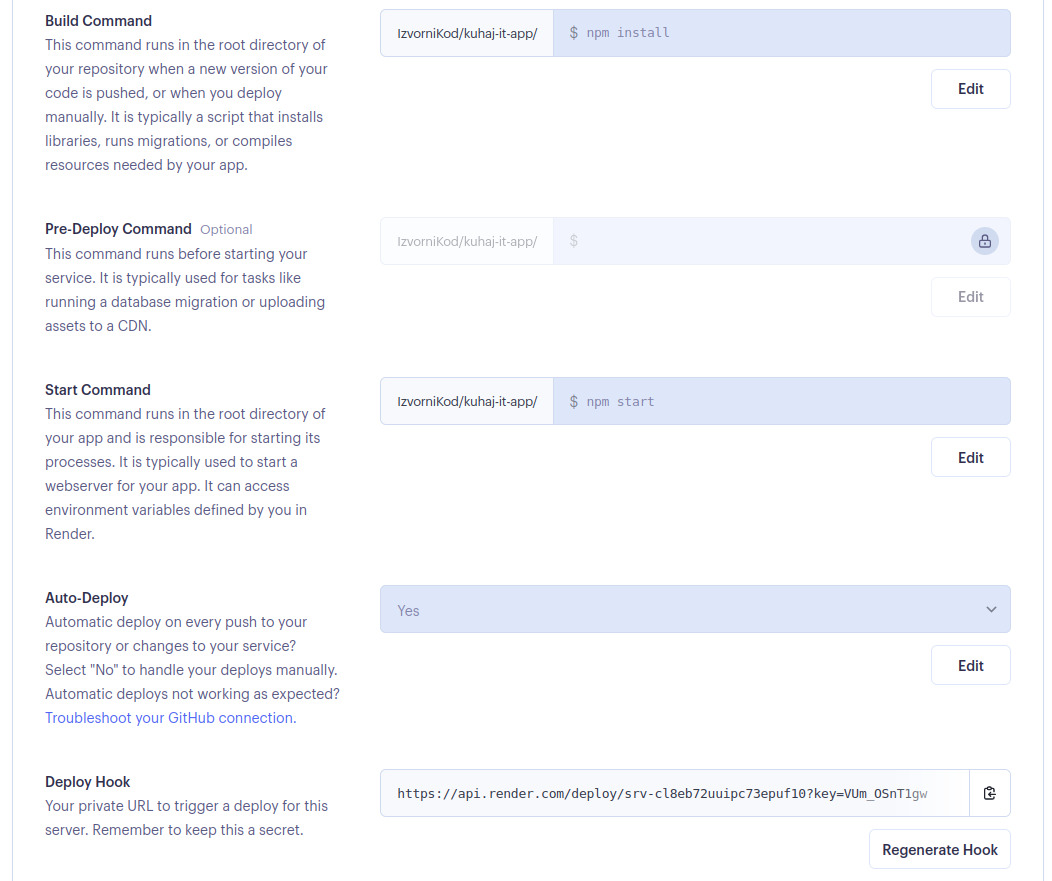
\includegraphics[scale=0.4]{slike/Render_FRONTEND_2.JPG} %veličina slike u odnosu na originalnu datoteku i pozicija slike
			\centering
			\caption{Postavke za postavljanje React web aplikacije, 2. dio}
			\label{Postavke za postavljanje React web aplikacije, 2. dio}
		\end{figure}
		
		Na gornjoj je slici vidljivo da smo za "naredbu izgradnje", naredbu koja će instalirati sve biblioteke, pokrenuti migracije i kompajlirati sve potrebno za ispravan rad naše React web aplikacije, odabrali naredbu "npm install".
		Ono što je još trebalo podesiti je naredba pokretanja, koju smo podesili na "npm start".
		Isto kao i kod podešavanja Spring Boot poslužitelja, odabrali smo opciju Auto-Deploy. \\
		
				\textbf{Postavljanje baze podataka} \\
				Iako nešto drugačije od "deploy-anja" Spring Boot poslužitelja i React web aplikacije, postavljanje PostgreSQL baze podataka na platformu Render također je izrazito jednostavno. \\
				Za početak, potrebno je na početnoj stranici stisnuti gumb New, a zatim odabrati opciju PostgreSQL, kako je prikazano na slici ispod.
				
				\begin{figure}[H]
			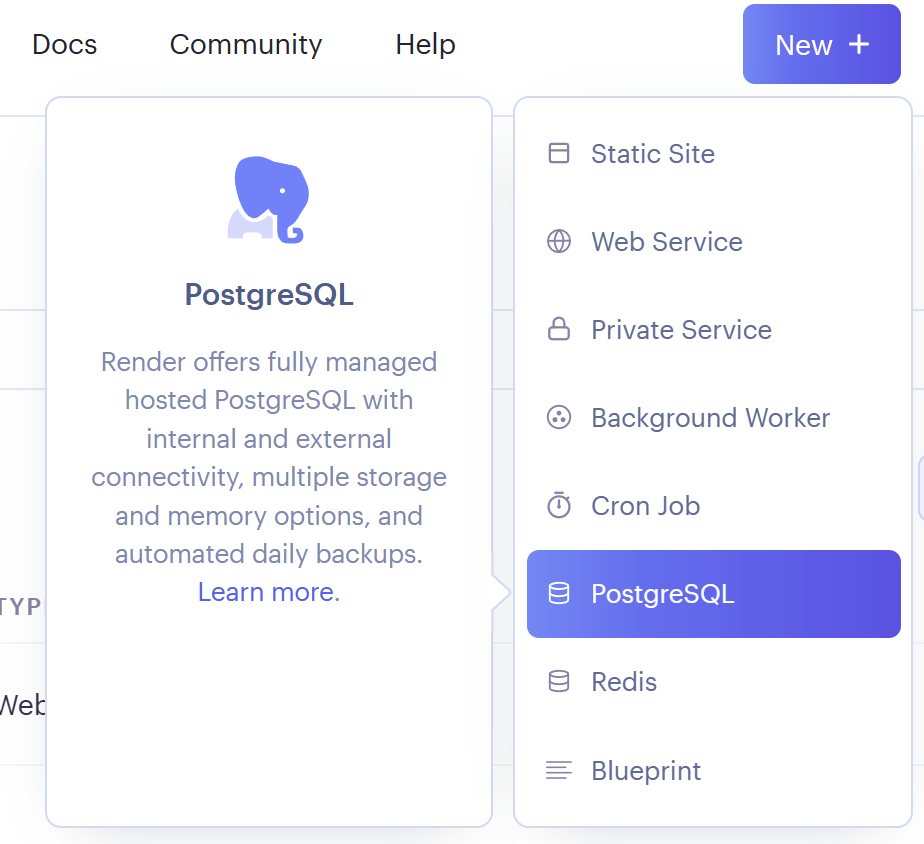
\includegraphics[scale=0.4]{slike/Render_PostgreSQL.PNG} %veličina slike u odnosu na originalnu datoteku i pozicija slike
			\centering
			\caption{Dodavanje nove PostgreSQL baze podataka}
			\label{Dodavanje nove PostgreSQL baze podataka}
		\end{figure}
		
		Odabirom opcije PostgreSQL, otvara se novi prozor na kojem je moguće unijeti razne podatke o bazi podataka: ime, korisnika, verziju PostgreSQL-a itd. Podatke koje smo mi unijeli prikazani su na slikama ispod.
		
			\begin{figure}[H]
			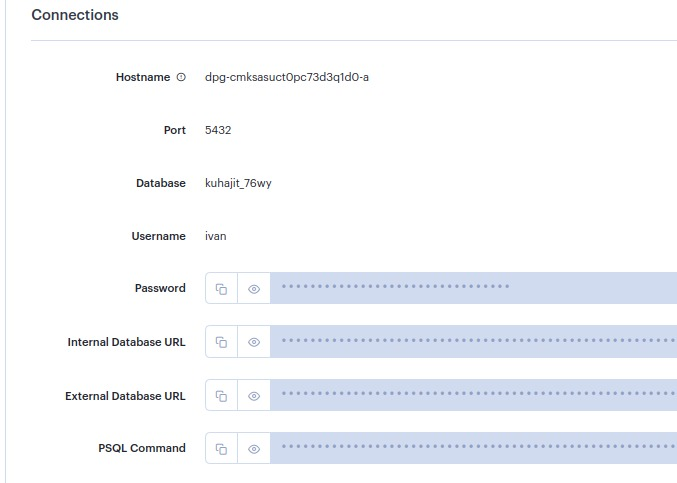
\includegraphics[scale=0.4]{slike/Render_DATABASE_1.JPG} %veličina slike u odnosu na originalnu datoteku i pozicija slike
			\centering
			\caption{Postavke baze podataka na Render-u, 1. dio}
			\label{Postavke baze podataka na Render-u, 1. dio}
		\end{figure}
		
		\begin{figure}[H]
			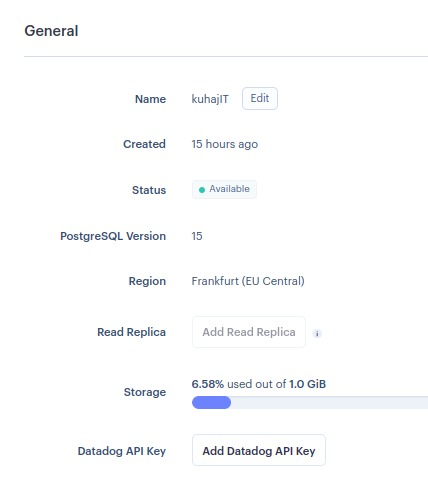
\includegraphics[scale=0.4]{slike/Render_DATABASE_2.JPG} %veličina slike u odnosu na originalnu datoteku i pozicija slike
			\centering
			\caption{Postavke baze podataka na Render-u, 2. dio}
			\label{Postavke baze podataka na Render-u, 2. dio}
		\end{figure}
		
		Postavka "Password" šifra je usera koja služi za spajanje na bazu i vidljiva je u datoteci application.properties, dok su polja Internal Database URL, External Database URL i PSQL Command generirana od strane platforme Render.
		
		Stvorena baza podataka je prazna, a mi ju moramo napuniti podacima. Skripta za izravno punjenje baze podataka (inicijaliziranje svih tablica i veza između njih te punjenje nekim testnim podacima) nalazi se u datoteci Script.sql, a mi smo ju pokretali izravno iz razvojnog okruženja Eclipse IDE.
		
				
	
		
	
	
	
		
		
		
		
		
		
		
		
		 
		
		
	    
	    
		
		
		
		
		
		
		
			
			\eject 